%%% Time-stamp: <mainrep.tex 19:57, 17 Jul 2016 by P Sunthar>
%%% $Log:$
% This document describes how to use iitbreport style
%********************************************************************

%\documentclass[11pt,a4paper,openright]{report}
\documentclass[twoside]{iitbreport}

%% Default spacing: 1.5
%% Default font size: 12pt
%% Default font: cmr

%%%%%%%%%%%%%%%%%%%%%%%%%%%%%%%%%%%%%%%%%%%%%%%%%%%%%%%%%%%%%%%%%%%%%
%% Prelims from RevelioBP paper

% \usepackage{cite}
% \usepackage{amsmath,amssymb,amsfonts}
\usepackage{algorithmic}
% \usepackage{graphicx}
% \usepackage{textcomp}
% \usepackage{bmpsize}
% \usepackage[dvipsnames]{xcolor}
% \usepackage{lipsum}
\usepackage{longtable}
\usepackage{cryptocode}
\usepackage{framed}
\usepackage{fancybox}
\usepackage{array}
\usepackage{mdframed}
\usepackage{enumitem}
% \usepackage{nameref}
\usepackage{upgreek}
% \usepackage{cases}
\usepackage{multirow}
% \usepackage{mathrsfs}
% \usepackage{dutchcal}
% \usepackage{eufrak}
% \usepackage{bbm}
% \usepackage[T1]{fontenc}
% \usepackage[utf8]{inputenc}
% \usepackage{tgadventor}
\usepackage[symbol]{footmisc}
\usepackage{caption,subcaption}
% \usepackage{subfigure}


\usepackage{pgfplots}
\pgfplotsset{compat=1.9}
\usetikzlibrary{spy}
\usetikzlibrary{external}
\usepgfplotslibrary{groupplots}
\tikzexternalize[prefix=plots/]

% \usepackage[colorlinks=true,urlcolor=black]{hyperref}

\newtheorem{theorem}{Theorem}
\newtheorem{lemma}{Lemma}
\newtheorem{corollary}{Corollary}
\newtheorem{definition}{Definition}

\def\BibTeX{{\rm B\kern-.05em{\sc i\kern-.025em b}\kern-.08em
    T\kern-.1667em\lower.7ex\hbox{E}\kern-.125emX}}




%%%%%%%%%%%%%%%%%%%%%%%%%%%%%%%%%%%%%%%%%%%%%%%%%%%%%%%%%%%%%%%%%%%



%% Selectively comment out sections that you want to be left out but
%% maintaining the page numbers and other \ref
\includeonly{%
  intro/introduction,
  prelims/crypto_prelims,
  lit/literature,
  expt/experimental,
  rnd/results, 
  dec,abs,pub,ack
}

%%% Some commonly used packages (make sure your LaTeX installation
%%% contains these packages, if not ask your senior to help installing
%%% the packages)

\usepackage{booktabs}
\graphicspath{{expt/}}

%%% Multibib package to be used for listing own publications.
\usepackage[resetlabels]{multibib}
\newcites{Pub}{List of Publications}


%%% Macro definitions for Commonly used symbols
\newcommand{\Rey}{\ensuremath{\mathrm{Re}}}
\newcommand{\avg}[1]{\ensuremath{\overline{#1}}}
\newcommand{\tenpow}[1]{\ensuremath{\times 10^{#1}}}
\newcommand{\pder}[2]{\ensuremath{\frac{\partial#1}{\partial#2}}}

% new \oset macro
\makeatletter
\newcommand{\oset}[3][0ex]{%
  \mathrel{\mathop{#3}\limits^{
    \vbox to#1{\kern-2\ex@
    \hbox{$\scriptstyle#2$}\vss}}}}
\makeatother

\newcounter{mylabelcounter}

\makeatletter
\newcommand{\labelText}[2]{%
#1\refstepcounter{mylabelcounter}%
\immediate\write\@auxout{%
  \string\newlabel{#2}{{1}{\thepage}{{\unexpanded{#1}}}{mylabelcounter.\number\value{mylabelcounter}}{}}%
}%
}
\makeatother

\newcommand{\vecb}[1]{\oset[-0.4ex]{\rightharpoonup}{\textbf{#1}}}
\newcommand{\vecnb}[1]{{\boldsymbol{#1}}}
\newcommand{\rgen}{\oset[1pt]{\hspace{3mm}\$}{\leftarrow}}


\newcommand{\Plus}{\raisebox{.20ex}{\normalsize\bf +}}
\newcommand{\plus}{\raisebox{.24ex}{\footnotesize +}}
\newcommand{\ToDo}[1]{[\textcolor{blue}{ToDo}: #1]}
\newcommand{\Rplus}{\RBw}
\newcommand{\RPlus}{\RB}
\newcommand{\proto}{$\Uppi_{\RBmath}$ }
\newcommand{\protow}{$\Uppi_{\RBmath}$}

\newcommand{\lang}{$\L_{\RBmath}$ }
\newcommand{\langw}{$\L_{\RBmath}$}

\newcommand{\R}{\textnormal{{\small \fontfamily{qag}\selectfont Revelio}} }
\newcommand{\RB}{\textnormal{{\small \fontfamily{qag}\selectfont RevelioBP}} }
\newcommand{\RBmath}{\textnormal{{\scriptsize \fontfamily{qag}\selectfont RevBP}} }
\newcommand{\Rw}{\textnormal{{\small \fontfamily{qag}\selectfont Revelio}}}
\newcommand{\RBw}{\textnormal{{\small \fontfamily{qag}\selectfont RevelioBP}}}
 
\newcommand{\N}{\mathbb{N}}
\newcommand{\F}{\mathbb{F}}
\newcommand{\E}{\mathscr{E}}
\newcommand{\Inf}{\mathcal{O}}
\newcommand{\Emat}{\mathbcal{E}}
\newcommand{\lvec}{\mathbcal{l}}
\newcommand{\rvec}{\mathbcal{r}}
\newcommand{\Z}{\mathbb{Z}}
\newcommand{\G}{\mathbb{G}}
\newcommand{\Rn}{\mathbb{R}}
\renewcommand{\P}{\mathcal{P}}
\newcommand{\V}{\mathcal{V}}
\newcommand{\C}{\mathcal{C}}
\renewcommand{\L}{\mathcal{L}}
\newcommand{\D}{\mathcal{D}}

\newcommand{\qed}{$\blacksquare$}

\newcommand{\protocolStart}{\begin{itemize}[leftmargin=*]}
\newcommand{\protocolEnd}{\end{itemize}}

\setlist[itemize]{leftmargin=0mm}
\setlist[enumerate]{leftmargin=1cm}

\newcommand{\pointsStart}{\begin{itemize}[leftmargin=*]}
\newcommand{\pointsEnd}{\end{itemize}}

\renewcommand{\thefootnote}{\fnsymbol{footnote}}
\colorlet{lightblue}{Blue!40}


\newtheorem{defn}{Definition}[section]


% Referencing macros
\newcommand{\Eqref}[1]{Equation~\eqref{#1}}
\newcommand{\Tabref}[1]{Table~\ref{#1}}
\newcommand{\Figref}[1]{Figure~\ref{#1}}
\newcommand{\Appref}[1]{Appendix~\ref{#1}}


\begin{document}
	
%%********************************Frontmatter***********************
% In frontmatter everything comes with roman numbering	
\pagenumbering{roman}
\setcounter{page}{1}

%*******************************************************************
%                         Title Page                            
%*******************************************************************
\title{Shorter, Privacy-Preserving Proof of Reserves Protocols for Cryptocurrency Exchanges}
\author{Suyash Bagad}

%% Print the date. Today's date comes by default, change it here to 
%% other date format, if required:

%\date{\today}
%\date{10 Mar 2016}


%% The type of the report can be set here

\reporttype{A Seminar Report}
%\reporttype{A Thesis}
%\reporttype{A Dissertation}
%\reporttype{A Project Report}

%% Name of the degree
\degree{Dual Degree (B.Tech \& M.Tech) in Electrical Engineering with Specialization in Communication \& Signal Processing}
%\degree{Master of Technology}


%% Department/Centre Name
\dept{Department of Electrical Engineering}

%% Supervisor and cosupervisor/excosupervisor are not essential parts
%% of a report title page, as it is your report!

%% But if you **have** to put it uncomment these
\supervisor{Prof. Saravanan Vijayakumaran}
%\cosupervisor{Co-super name}
% \excosupervisor{External Supervisor}

%% Roll number
\rollnum{Roll No. 15D070007}

\maketitle

%*******************************************************************
%                         Copyright Page                          
%******************************************************************* 
%\mycopyright                    

%*******************************************************************
%                         Dedication Page                         
%*******************************************************************
\dedication[Dedicated to \ldots]        
%\addintoc{Dedication}

%*******************************************************************
%                        Certificate Page                         
%*******************************************************************
%\makecertificate[change title name]{report type} 
% \makecertificate{seminar report} 
%\makecertificate{thesis}
\makecertificate{dissertation}
%\makecertificate{project report}

%\addintoc{Certificate}

%*******************************************************************
%                         Approval Sheet                         
%*******************************************************************
%\makeapproval{thesis}
%\makeapproval{dissertation}

%*******************************************************************
%                          Declaration                           
%*******************************************************************
%==================================dec.tex================================
%
\begin{Declaration}
\noindent
I declare that this written submission represents my ideas in my own words and where others' ideas or words have been included, I have adequately cited and referenced the original sources. I declare that I have properly and accurately acknowledged all sources used in the production of this report. I also declare that I have adhered to all principles of academic honesty and integrity and have not misrepresented or fabricated or falsified any idea/data/fact/source in my submission. I understand that any violation of the above will be a cause for disciplinary action by the Institute and can also evoke penal action from the sources which have thus not been properly cited or from whom proper permission has not been taken when needed.

%
%
%
%
%
%
%

\DecSign[24 June 2020]



%
\end{Declaration}
%========================================================================
















 
%\addintoc{Declaration}

%******************************************************************
%                          Abstract                             
%******************************************************************  
%============================= abs.tex================================
\begin{Abstract}
The rise of cryptocurrencies began with the inception of Bitcoin in 2009. Since
then, several cryptocurrencies with better privacy and security guarantees are being
developed. Cryptocurrencies gained popularity among general masses with the establishment of cryptocurrency exchanges.
Also known as digital currency exchanges or crypto exchanges, they are essentially businesses that allow customers to trade
cryptocurrencies or digital currencies for other assets including conventional fiat
money or different digital currencies. 
From a customer point of view, exchanges not only made owning cryptocurrencies possible to non-miners but also provided them with fast trading platforms for transactions within cryptocurrencies and fiat.
Customers were also provided with custodial wallets freeing them from the hassle of storing and remembering private keys.
In the early days of cryptocurrency, crypto exchanges were very few and less-known, but not too long ago their number increased dramatically and they became an integral part of the cryptoeconomic ecosystem. 
They were responsible for the boost in the transaction volumes of the vast majority of the cryptocurrency sales and liquidity.

The downside of such cryptocurrency exchanges is that they are required to
store sensitive information of customers like the private keys and account balances.
If in case an exchange is hacked, it might result in loss of customer-owned cryptocurrency assets.
There have been many high-profile hacks over the years, many of which went unnoticed for some time \cite{Cryptohacks}.
Although having a fool-proof method to avoid such hacks might be a difficult task, proof of reserves is one way to uphold the trust of customers.
A proof of reserves is the guarantee by the exchange that it owns reserves at least as much as its total liabilities towards customers. 
In this way, even after cases of hacking, the exchange could repay its liabilities to the customers.

The simplest way to publish a proof of reserves for an exchange is to reveal all the addresses or account details it owns so that the customers are convinced about the assets owned by the exchange.
Another way could be to send all the reserves it owns from all its addresses to a single addresses it owns.
If amounts involved in a transaction are public as in the case of Bitcoin, such a self-transaction would be a proof of the exchange's reserves.
For example, in 2011, Mt.~Gox cryptocurrency exchange transferred 424,242 bitcoins from its wallets to a previously revealed Bitcoin address \cite{MtGoxWikipedia}.
However, such proofs of reserves do not preserve the privacy of the exchanges. 
Information of an exchange's addresses or accounts and the total assets it owns are crucial for aspects of its business.
Exchanges naturally would not be in a position to compromise such critical information as a part of proofs of reserves.
The main challenge in design of proofs of reserves is to preserve privacy and confidentiality of exchanges but at the same time convince customers about an exchange's actual asset ownership.
Regaining \textit{trust} of the customers without compromising exchanges' \textit{privacy} is the primary motivation behind the design of better proofs of reserves. 
Advanced cryptographic techniques make it possible to design proofs of reserves which reveal \textit{nothing} beyond an assertation of the form:
\begin{center}
    \texttt{Exchange ABC owns ? amount of Y cryptocurrency and here is a proof $\Pi$ for customers to verify.}
\end{center}
Note that here we do not intend to reveal even the total amount. 
The proof $\Pi$ is a cryptographic tool known as a \textit{Non-Interactive Zero-Knowledge} proof.

In this work, we study the existing proof of reserves protocols for privacy-centric cryptocurrencies Grin, Beam and Monero.
The existing proof of reserves protocols possess some shortcomings which becomes a hurdle in their practical deployment.
With an aim to alleviate limitations of previously designed proofs of reserves, we design novel proofs of reserves for crypto exchanges supporting the above cryptocurrencies.
Our protocols are shorter and privacy enhancing in comparison to the existing state-of-the-art proofs of reserves.
We also implement the protocols we design as well as the previous state-of-the-art protocols for comparison and show feasibility in practical deployment of our protocols.
We believe that our work on proof of reserves could be well adopted by crypto exchanges and benefit several of their customers.
Furthermore, our work also opens up avenues of exploration of establishing trust without compromising privacy or anonymity in a more general setting.
We are hopeful that this work acts as a small but crucial contribution towards the goal of establishing a \textit{trustless, decentralized economy.}
%
%
%
%
%
\end{Abstract}
%=======================================================================

                    

%******************************************************************
%                         Contents list                         
%******************************************************************
%\figurespagefalse
%\tablespagefalse
\makecontents % Creats toc, lof, and lot

%******************************************************************
%                        Notations                              
%******************************************************************
\notations[4cm]{List of Symbols}      

%%********************************Mainmatter***********************
% In mainmatter everything comes with arabic numbering	
\cleardoublepage
\setcounter{page}{1}
\pagenumbering{arabic}

%******************************************************************
%                         Chapters                           
%****************************************************************** 

\newcommand{\etas}{\ensuremath{\eta_{\mathrm{s}}}}


\chapter{Introduction}

The rise of cryptocurrencies have openend up unending possibilities of how minimal or no trust based systems could be established owing to decentralization.
The concept of blockchain was introduced with the founding of Bitcoin by Satoshi Nakamoto \cite{Nakamoto2009}.
Satoshi Nakamoto proposed and implemented idea of a consensus based, trustless, truly peer-to-peer system for financial transactions.  
Notwithstanding an intrumental step towards establishing a decentralized and a trustless system, Bitcoin has several practical limitations with regards to privacy, security and scalability \cite{Conti2018}.   
This led to the development of more privacy and anonymity focussed cryptocurrencies like Monero \cite{Saberhagen2013} and Zcash \cite{Sasson2014}.
Grin \cite{GrinWebsite} and Beam \cite{BeamWebsite} are two relatively new projects which are backed by the MimbleWimble protocol \cite{Poelstra2016} and claim to promise scalability, anonymity and fungibility all at once.
The rise in privacy-centric cryptocurrencies further led to growth in popularity of cryptocurrencies not only among investors but also common people.


\section{What is a Blockchain?}
\label{scn:blockchain}

The concept of a Blockchain originates from the idea of having a decentralized, publicly visible and trust-free ledger.
The term \textit{blockchain} was first coined by Satoshi Nakamoto, the creator of Bitcoin \cite{Nakamoto2009}.
In literal terms, a blockchain implies that blocks containing financial transactions would be added to a publicly verifiable ledger in a timely manner, forming a \textit{chain} of \textit{blocks}.
We expand on the need and the basic idea of a decentralized ledger in the following subsection.

\subsection{Decentralized Ledger}

A ledger is a principal book of records which keeps a track of all transactions measured in terms of a monetary unit. Bitcoin is a decentralized, public ledger, decentralized because there is no trusted third party controlling the ledger and public because anyone with bitcoin can participate in the network, receive and send bitcoins, and even hold a copy of this ledger (essentially, the history of all transactions) if they want to. In that sense, the ledger is "non-trusted" and transparent to public. As opposed to such a decentralized ledger setup, traditional banks use centralized ledger system where each bank has it's own ledger visible only to the concerned user.\\ 

\begin{figure}[h!]
    \centering
    \begin{subfigure}[b]{0.5\textwidth}
        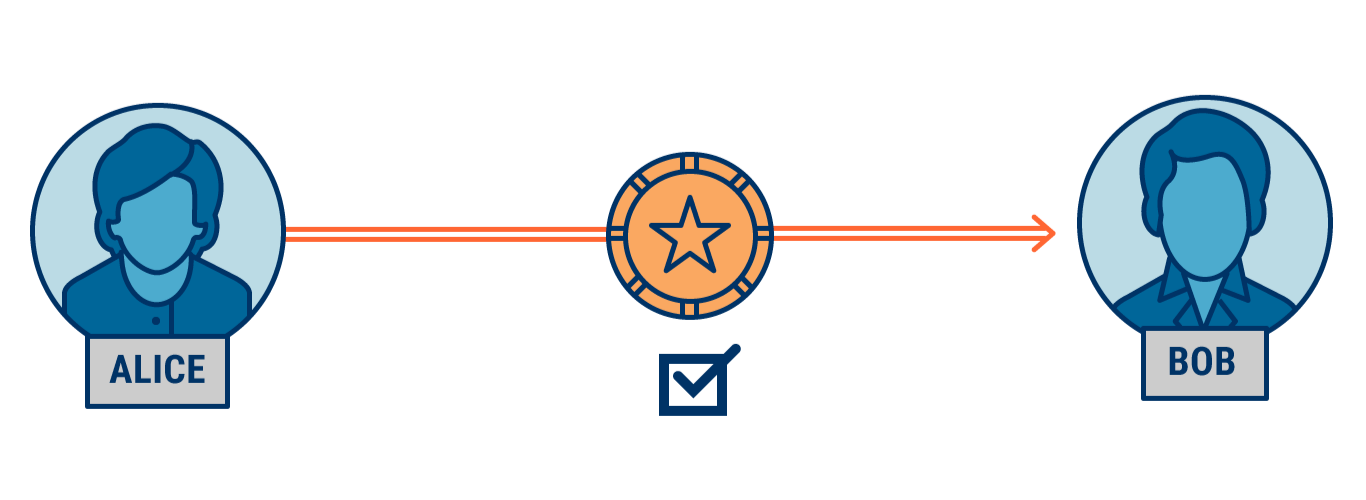
\includegraphics[width=\textwidth]{Figures/blockchain1.png}
        \caption{A physical transaction}
        \label{fig:bc1}
    \end{subfigure}
    ~
    \begin{subfigure}[b]{0.5\textwidth}
        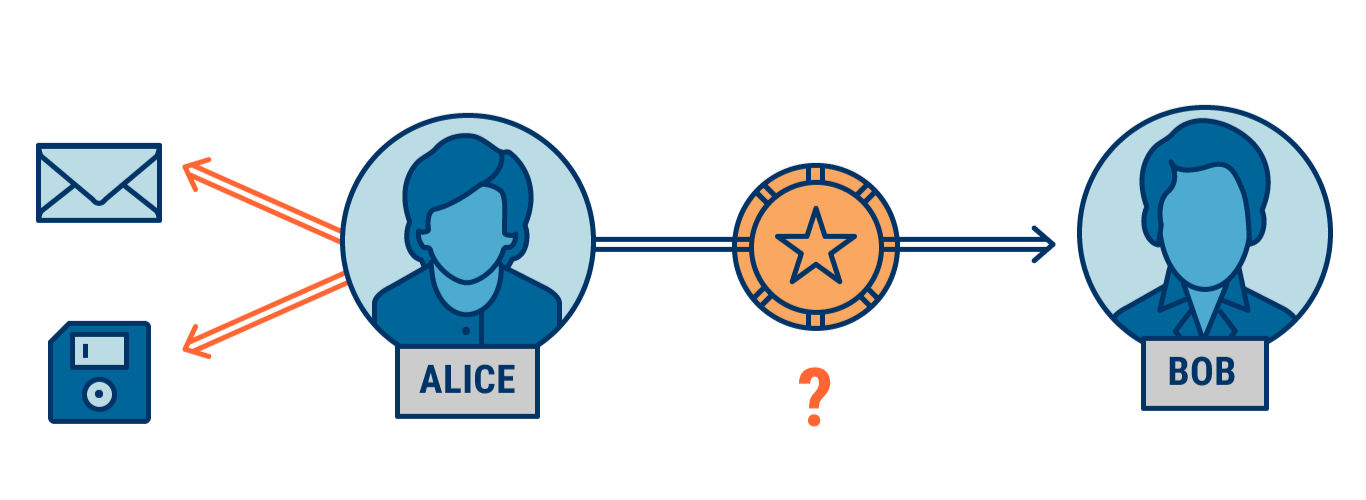
\includegraphics[width=\textwidth]{Figures/blockchain2.png}
        \caption{A digital transaction}
        \label{fig:bc2}
    \end{subfigure}
    ~
    \begin{subfigure}[b]{0.5\textwidth}
        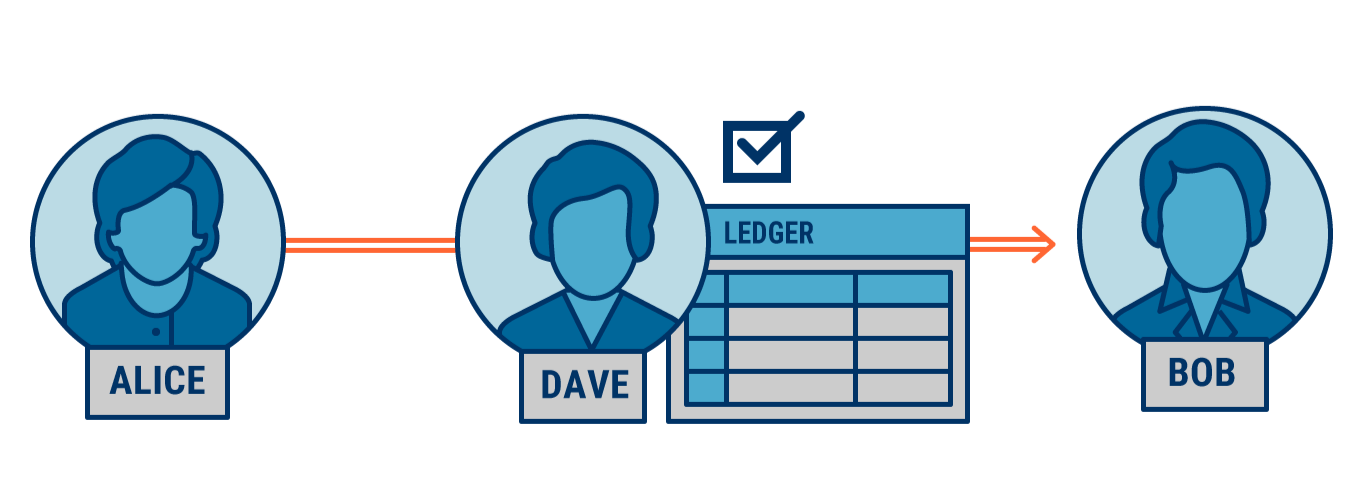
\includegraphics[width=\textwidth]{Figures/blockchain3.png}
        \caption{A digital transaction with ledger}
        \label{fig:bc3}
    \end{subfigure}
    ~
    \begin{subfigure}[b]{0.7\textwidth}
        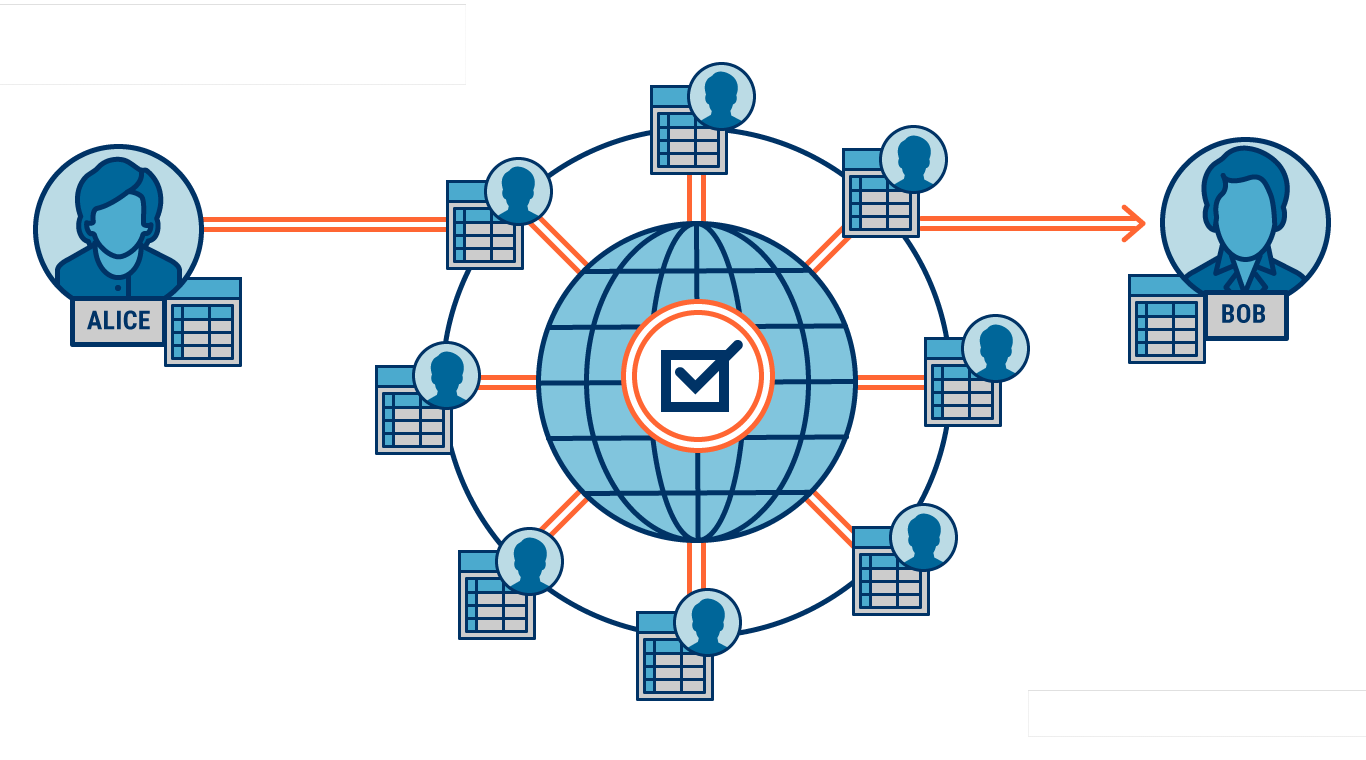
\includegraphics[width=\textwidth]{Figures/blockchain4.png}
        \caption{A decentralized ledger}
        \label{fig:bc4}
    \end{subfigure}
    \caption{Understanding decentralized ledger}
    \label{fig:bc}
\end{figure}

In reference to Figure\footnote{Credits: \url{https://www.cbinsights.com/research/what-is-blockchain-technology/}}
\ref{fig:bc1}, in a physical transaction, the Alice hands Bob a physical arcade coin. Bob now has one coin, and Alice has zero. The transaction is complete. 
If the same transaction is to be performed digitally (Figure \ref{fig:bc2}), Alice would send a string of some bits (corresponding to the desired amount) to Bob. 
Now, since it is just a string of bits, what is the guarantee that Alice would not reproduce that same string of bits in her mail or hard-disk?
If this happens, it would mean that although Alice sent Bob the amount, Alice still possesses the same amount. 
This clearly is a violation.
To tackle this, we must have a ledger or a record of all transactions between Alice and Bob. 
When Alice gives Bob the digital token, the ledger records the transaction (Figure \ref{fig:bc3}). 
Bob has the token, and Alice does not. Let us call the one who maintains this ledger as Dave.
This setup assumes that Dave is a trusted middleman for maintaining ledger. 
Now, what if Alice bribes Dave to erase her transaction? What if Dave decides to charge a fee that neither Alice or Bob want to pay? 
What happens when Alice and Bob cannot trust the third party? This results in a decentralized and public ledger system (Figure \ref{fig:bc4}). 
When a lot of people have a copy of the same ledger, it becomes very difficult to tamper the system and cheat. 
This works because everyone is holding a copy of the same digital ledger and more the number of trusted people holding this ledger, the stronger it becomes.


Blockchain technology offers a way for untrusted parties to reach a consensus on a common digital history. The World Bank defines Blockchain as follows \cite{natar17}:

\begin{definition}[Blockchain]
    A 'blockchain' is a particular type of data structure used in some distributed ledgers
    which stores and transmits data in packages called "blocks" that are connected to each
    other in a digital 'chain'. 
\end{definition}

Blockchains employ cryptographic algorithms to record and synchronize data across a network in an unchangeable manner. The \textit{state} of the Blockchain is the current status of the ledger visible to public. 
In case of Bitcoin, any independent observer can verify the state of the blockchain as well as the validity of all the transactions on the ledger.
This is a \textit{serious} limitation for Bitcoin and could possibly prohibit many use cases.
As an example, if employees of a company were to receive their salaries in bitcoin, would they agree if their salaries were published on the public blockchain? 
This naturally demands for a transaction system which preserves \textit{anonymity} and \textit{confidentiality}.


\section{Notion of Privacy on a Blockchain}

The very concept of having all the information about transactions (predominantly financial) public via a distributed ledger or a blockchain demands for privacy and anonymity of the users.
Before we talk about privacy on the blockchain, it is necessary to understand what we do mean by terms like \textit{privacy} and \textit{anonymity}.
Modern day cryptography is based on the following primary functions \cite{kesler98}:
\begin{enumerate}
    \item[(i)] \textit{Privacy/confidentiality}: To ensure that no one can read or access the message except the intended receiver
    \item[(ii)] \textit{Authentication}: Proving one's identity
    \item[(iii)] \textit{Integrity}: Ensuring that the message intended to be received by the receiver is not altered in the path
    \item[(iv)] \textit{Non-repudiation}: A protocol for checking if a message was actually generated by the sender
    \item[(v)] \textit{Key exchange}: The protocol which determines how key(s) are shared between the sender and the receiver
\end{enumerate}

All of the above functions form an necessary part of a cryptographic system. A well-designed system ensures all of the above functions are taken care of considering the computational bounds for carrying out any protocol.
In a confidential transaction, it is desirable to have \textit{confidentiality} and \textit{anonymity}. 
This means that in a valid confidential transaction, the identity of the sender and receiver must be confidential and the amounts transferred must also be hidden. 
The idea of having such private transactions in digital currencies could be traced back to David Chaum's work on blind signatures \cite{chaum82}.
A similar concept of privacy is required in the blockchain framework. 
The digital assets owned by users must not be publicly visible.
There should be a mechanism to unlink the identity of a user with his or her digital identity, i.e. public key address. 
The interaction between the sender and the receiver in a transaction must not reveal anything to them other than the amounts being transferred.
A user must not be able to reuse his or her digital assets. 
Making the transactions digital and public at the same time brings about several challenges in ensuring that the above requirements are being satisfied.
Active research is still being pursued in the direction of not only solving such practical problems but to do them efficiently and in a scalable manner.

\section{Cryptocurrency Exchanges}

The rise of cryptocurrencies began with the inception of Bitcoin in 2009. Since
then, several cryptocurrencies with better privacy and security guarantees are being
developed. Cryptocurrencies gained popularity among general masses with the establishment of cryptocurrency exchanges.
Also known as digital currency exchanges or crypto exchanges, they are essentially businesses that allow customers to trade
cryptocurrencies or digital currencies for other assets including conventional fiat
money or different digital currencies. 
From a customer point of view, exchanges not only made owning cryptocurrencies possible to non-miners but also provided them with fast trading platforms for transactions within cryptocurrencies and fiat.
Customers were also provided with custodial wallets freeing them from the hassle of storing and remembering private keys.
In the early days of cryptocurrency, crypto exchanges were very few and less-known, but not too long ago their number increased dramatically and they became an integral part of the cryptoeconomic ecosystem. 
They were responsible for the boost in the transaction volumes of the vast majority of the cryptocurrency sales and liquidity.

\subsection{Hacks and Frauds of Exchanges}

The downside of cryptocurrency exchanges is that they are required to
store sensitive information of customers like the private keys and account balances.
If in case an exchange is hacked, it might result in loss of customer-owned cryptocurrency assets.
There have been many high-profile hacks over the years, many of which went unnoticed for some time \cite{Cryptohacks}.
In 2014, one of the biggest Bitcoin exchanges Mt.Gox lost almost 750,000 of its customers' bitcoins and around 100,000 of its own bitcoins, totaling around 7\% of all bitcoins back then, and worth around \$473 million, leading to filing of bankruptcy.
There have been cases where exchanges lure customers into buying digital assets in return for fiat currency, but do not allocate any digital assets in reality.
Such exit scams by exchanges have led to huge losses of customer and investor funds \cite{Robert2020}.

Although having a fool-proof method to avoid such hacks might be a difficult task, proof of solvency is one way to uphold the trust of customers.
A proof of solvency is the guarantee by the exchange that it owns reserves at least as much as its total liabilities towards customers. 
In this way, even after cases of hacking, the exchange could repay its liabilities to the customers.


\section{Proof of Solvency}

An exchange is said to be solvent if it owns assets at least as much as its liabilities.
An exchange proving solvency convinces its customers that in an unfortunate case of a hack or a fraud, it could reimburse the lost customer funds through its own assets.
A proof of solvency consists of two parts: proof of reserves and proof of liabilities.
The former proves the assets owned by the exchange while the latter shows the total liabilities of the exchange towards its customers.

The challenge in designing proof of solvency is to maintain privacy of the exchange as well as the customers.
Proof of reserves protocols in \cite{Dagher2015,Dutta2019a,Dutta2019b} publish a Pedersen commitment to the total assets owned by the exchange.
Pedersen commitments are a cryptographic way of hiding secret messages or amounts. We will describe Pedersen commitments in detail in the next chapter.
Suppose an exchange publishes $C_{\text{res}}$ as a Pedersen commitment to its total reserves $a_{\text{res}}$.
Similarly, it could publish a Pedersen commitment to its total liabilities $a_{\text{liab}}$ as $C_{\text{liab}}$ using customer data as described in \cite{Dagher2015}.
However, this proof of reserves in \cite{Dagher2015} requires each customer to individually verify that his or her amount is included in the proof of liabilities.
If a customer fails to verify his or her amount, the exchange in principle could hide the particular customer's data to shrink its liabilities.
Chalkias \textit{et al}. \cite{Chalkias2020} recently proposed a scheme called Distributed Auditing Proofs of Liabilities (DAPOL) which addresses this concern. 
% DAPOL uses deterministic sparse Merkle tree combined with range proofs on the commitment to each customer's amount and a Pedersen commitment to $a_{\text{liab}}$. 
DAPOL uses private information retrieval to ensure the inclusion proof by every customer.
Therefore, given the Pedersen commitments to reserves and liabilities of an exchange, it can prove solvency by proving that the quantity $C_{\text{res}} \cdot C_{\text{liab}}^{-1}$ commits to a non-negative amount and thus, $a_{\text{res}} - a_{\text{liab}} \ge 0$.
This suffices because $C_{\text{res}} \cdot C_{\text{liab}}^{-1}$ is a Pedersen commitment to $a_{\text{res}} - a_{\text{liab}}$ due to the homomorphic property of Pedersen commitments.

\subsection{Proof of Reserves}

A proof of reserves protocol is used by a cryptocurrency exchange to prove that it owns a certain amount of cryptocurrency. 
If privacy of the amount or outputs owned by the exchange is not an issue, then proving reserves involves a straightforward proof of the ability to spend the exchange-owned outputs (for example, see \cite{BlockstreamProofOfReserves}). 
The simplest way to publish a proof of reserves for an exchange is to reveal all the addresses or account details it owns so that the customers are convinced about the assets owned by the exchange.
Another way could be to send all the reserves it owns from all its addresses to a single addresses it owns.
If amounts involved in a transaction are public as in the case of Bitcoin, such a self-transaction would be a proof of the exchange's reserves.
For example, in 2011, Mt.~Gox cryptocurrency exchange transferred 424,242 bitcoins from its wallets to a previously revealed Bitcoin address \cite{MtGoxWikipedia}.
Information of an exchange's addresses or accounts and the total assets it owns are crucial for aspects of its business.
Thus, non-private proof of reserves protocols are unlikely to be adopted by exchanges as they may reveal business strategy. 
Privacy-preserving proof of reserves protocols have been proposed for Bitcoin \cite{Decker2015,Dagher2015}, Monero \cite{Dutta2019a}, and MimbleWimble \cite{Dutta2019b}. 
In fact, the protocols proposed by Decker \textit{et al} \cite{Decker2015} and Dagher \textit{et al} \cite{Dagher2015} go one step further and give a privacy-preserving proof of solvency, i.e.~they prove that the reserves owned by the exchange exceed its liabilities towards its customers. 
However, the work in \cite{Decker2015} relies on a trusted hardware assumption. And the proof of liabilities protocol in \cite{Dagher2015} is secure only if every exchange customer checks the proof. 
In general, it seems that designing proof of reserves protocols is easier than designing proof of liabilities protocols as the former depend only the blockchain state while the latter depend on the exchange's private customer data.
% An exchange can reduce its reported liabilities by censoring its customer list.

Even without a robust proof of liabilities protocol, a privacy-preserving proof of reserves protocol based on homomorphic commitments is valuable. 
% For example, the proof of reserves protocols in \cite{Dagher2015,Dutta2019a,Dutta2019b} generate a Pedersen commitment $C_{\text{res}}$ to the amount of reserves. 
Exchanges can easily prove that $C_{\text{res}}$ is a commitment to an amount which exceeds a base amount $a_{\text{base}}$. While the base amount may not be exactly equal to the total liabilities of the exchange, it can be based on the trade volume data published by the exchange \cite{Coinmarketcap}. 
This technique will help early detection of exchange hacks and exit scams. 
For example, in Februrary 2019 the Canadian exchange QuadrigaCX claimed that it had lost access to wallets containing customer funds due to the death (in December 2018) of their CEO who had sole custody of the corresponding passwords and keys. But an official investigation found that the wallets had been empty since April 2018, several months before the CEO's death \cite{QuadrigaCXEmpty, EYThirdReport}. This discrepancy would have been detected earlier if the exchange had been required to give perioidic proofs of reserves.
Realising the importance of proof of reserves as a tool in raising customer confidence in crypto-exchanges leads us to the need for building better proofs in terms of privacy, scalability and performance.    

The main challenge in design of proofs of reserves is to preserve privacy and confidentiality of exchanges but at the same time convince customers about an exchange's actual asset ownership.
Regaining \textit{trust} of the customers without compromising exchanges' \textit{privacy} is the primary motivation behind the design of better proofs of reserves. 
Advanced cryptographic techniques make it possible to design proofs of reserves which reveal \textit{nothing} beyond an assertation of the form:
\begin{center}
    \textit{Exchange X owns ? amount of the cryptocurrency Y.}
\end{center}
Note that here we do not intend to reveal even the total amount. 
A publicly verifiable proof backing up such a claim is a cryptographic tool known as a \textit{Non-Interactive Zero-Knowledge} proof.

\section{Organization of the Thesis}

After motivating the problem we are trying to address in this work, we will briefly describe the cryptographic primitives necessary to understand our work in Chapter \ref{chap:crypto_prelims}.
In Chapter \ref{chap:revBP}, we start with outlining the details of Grin and existing state-of-the-art proof of reserves protocol for MimbleWimble-based cryptocurrencies. 
We describe \RB - a novel proof of reserves protocol for MimbleWimble-based cryptocurrencies in Chapter \ref{chap:revBP} along with its security properties.
We present the Grin outputs' amount confidentiality analysis in Chapter \ref{chap:grin-ub}.
Finally, we put forth all the security proofs in the Appendix.  


%%


%%% Local Variables: 
%%% mode: latex
%%% TeX-master: "../mainrep"
%%% End: 

\chapter{Cryptographic Preliminaries}

Before delving into the details of \RPlus protocol, let us equip ourselves with some background knowledge about the math of cryptocurrencies.


\section{Notation}
Let $\mathcal{G} = \{ \G, q, g \}$ be the description of a cyclic group $\G$ of prime order $q$ with generator $g$ of $\G$. Let $h\in \G$ be another random generator of $\G$ such that the discrete logarithm relation between $g$ and $h$ is not known. Let
$\G^n$ and $\Z^n_q$ be the $n$-ary Cartesian powers of sets $\G$ and $\Z_q$ respectively.
%TODO: Check the second part of the following statement.
% Yes, it is.
Group elements which are Pedersen commitments are denoted by uppercase letters and randomly chosen group elements are denoted by lowercase letters.
% TODO: Check if the following statement is true after the rewrite.
% It is true and necessary too. Matrix description not necessary, so removing it.
Bold font denotes vectors.
Inner product of two vectors $\textbf{a}, \textbf{b} \in \Z_q^n$ is defined as $\langle \textbf{a},\textbf{b} \rangle \coloneqq \sum_{i=1}^{n} a_i \cdot b_i$ where $\textbf{a}=(a_1,\dots, a_n), \textbf{b}=(b_1,\dots,b_n)$. Further, Hadamard and Kronecker products are defined respectively as, $\textbf{a} \circ \textbf{b} \coloneqq (a_1 \cdot b_1, \dots, a_n \cdot b_n) \in \mathbb{Z}_q^n$, $\textbf{a} \otimes \textbf{c} \coloneqq (a_1 \textbf{c}, \dots, a_n \textbf{c}) \in \mathbb{Z}_q^{nm}$ where $\textbf{c} \in \mathbb{Z}_q^m$. For a base vector $\textbf{g} = (g_1, \dots, g_n) \in \G^n$, vector exponentiation is defined as $\textbf{g}^{\textbf{a}} = \prod_{i=1}^{n}g_i^{a_i} \in \G$. For a scalar $u \in \Z_q^{\ast}$, we denote its consecutive powers in the form of a vector $\vecnb{u}^{n} \coloneqq (1, u, u^2, \dots, u^{n-1})$.
To represent the exponentiation of all components of a vector $\textbf{a}$ by the same scalar $k \in \Z_q$, we use $\textbf{a}^{\circ k}$ to mean $(a_1^k, a_2^k, \ldots,a_n^{k})$.
If an element $a$ is chosen uniformly from a set $A$, such a choice is denoted by $a \rgen A$.
We denote the relation \emph{Relation} using the specified input and witness as $\{ (Public \ Input; \ Witness): Relation \}$.
We refer to $\mathcal{A}$ as a \textsf{PPT} adversary which is a probabilistic Turing Machine that runs in polynomial time in the security parameter $\lambda$.
An \emph{interactive proof} for the decision problem $\pi$ is described as follows:
\begin{enumerate}
    \item There are two participants, a \textcolor{blue}{prover} $\P$ and a \textcolor{blue}{verifier} $\V$.
    \item The proof consists of a specified number of rounds.
    \item In the beginning, both participants get the same input.
    \item In each round, the verifier challenges the prover, and the prover responds
    to the challenge.
    \item Both the verifier and the prover can perform some private computation.
    \item At the end, the verifier states whether he was convinced or not.
\end{enumerate}


\section{Assumptions}
\begin{defn}[Discrete Log Relation]
    For all PPT adversaries $\mathcal{A}$ and for all $n\ge2$, $\exists$ a negligible function $\mu (\lambda)$ s.t
    \begin{equation*}
        \Pr 
        \Big[
        \begin{tabular}{ll}
             $\G = Setup(1^{\lambda}), g_1, \dots, g_n \leftarrow \ \G$ ;
             &
             \multirow{2}{*}{$\text{:} \exists a_i \neq 0 \wedge \prod_{i=1}^{n} g_{i}^{a_i} = 1$}\\
             $a_1, \dots, a_n \in \ \Z_p \leftarrow \mathcal{A}(\G, g_1, \dots, g_n)$
             & 
        \end{tabular}
        \Big] 
      \leq \mu(\lambda)
    \end{equation*}
   
    \vspace{0.2mm}
\end{defn} 
We say $\prod_{i=1}^{n} g_{i}^{a_i} = 1$ is a non trivial discrete log relation between $g_1, \dots, g_n$. If the Discrete Log Relation assumption stands, it implies that no \textsf{PPT} adversary can find a non-trivial relation between randomly chosen group elements. 

We use additional cryptographic assumptions such as Decisional Diffie-Hellman and its variants as described in \cite{Lai2019}.

\section{Cryptographic Commitments}

\begin{defn}[Commitments]
    A non-interactive commitment consists of two PPT algorithms {\normalfont(Setup, Com)}. For a message $x \in {\normalfont \textbf{M}_{pp}}$ (message space), the algorithm proceeds as follows:
    \begin{itemize}
    \setlength\itemsep{0.3em}
        \item public parameters $pp \leftarrow {\normalfont Setup}(1^{\lambda})$ for security paramter $\lambda$
        \item {\normalfont Com}$_{pp} : {\normalfont \textbf{M}_{pp}} \times {\normalfont \textbf{R}_{pp}} \rightarrow {\normalfont \textbf{C}_{pp}}$, 
        where ${\normalfont \textbf{R}_{pp}}$ is randomness space
        \item $r \leftarrow {\normalfont \textbf{R}_{pp}}$ and compute {\normalfont \textbf{com}} = {\normalfont Com}$_{pp}(x;r)$
    \end{itemize}
\end{defn}

\begin{defn}[Homomorphic Commitments]
    A homomorphic commitment is a non-interactive commitment such that ${\normalfont \textbf{M}_{pp}}$, ${\normalfont \textbf{R}_{pp}}$, ${\normalfont \textbf{C}_{pp}}$ are all abelian groups, and $\forall \ x_1, x_2 \in {\normalfont \textbf{M}_{pp}}, r_1, r_2 \in {\normalfont \textbf{R}_{pp}}$, we have 
\end{defn}
\begin{equation*}
    \text{Com}(x_1; r_1) + \text{Com}(x_2; r_2) = \text{Com}(x_1+ x_2; r_1+r_2)
\end{equation*}

\begin{defn}[Hiding Commitment]
    A commitment scheme is said to be hiding if for all PPT adversaries $\mathcal{A}$, $\exists \mu(\lambda)$, a negligible function such that,  
\end{defn}
\begin{equation*}
        \Bigg|
        \Pr
        \Bigg[
        \begin{tabular}{c | l}
             \multirow{3}{*}{$\textit{b'=b}$} 
             &
             $\textit{pp} \leftarrow \text{Setup}(1^{\lambda})$;\\
             &
             $(\textit{x}_0,x_1) \in \text{\textbf{M}}_{pp}^2 \leftarrow \mathcal{A}(pp), \
             b \leftarrow \{0,1\}, \ 
             r \leftarrow \text{\textbf{R}}_{pp},$ \\
             &
             $\textbf{com} = Com(\textit{x}_b; r),\ b' \leftarrow \mathcal{A}(pp, \ \textbf{com})$
        \end{tabular}
        \Bigg]
        - \frac{1}{2}
        \Bigg|
        \leq \mu(\lambda)
\end{equation*}
\textit{where the probability is over $b', r, Setup \ \text{and} \ \mathcal{A}$. For perfectly hiding schemes, $\mu(\lambda)=0$.}


\begin{defn}[Binding Commitment]
    A commitment scheme is said to be binding if for all PPT adversaries $\mathcal{A}$, $\exists \mu(\lambda)$, a negligible function such that,
\end{defn}
\begin{equation*}
        \Pr 
        \Bigg[
        \begin{tabular}{c | c}
             \multirow{2}{*}{$\text{Com}(\textit{x}_0;r_0)= \text{Com}(\textit{x}_1;r_1) \wedge x_0 \neq x_1$} 
             &
             $\textit{pp} \leftarrow \text{Setup}(1^{\lambda})$,\\
             &
             $\textit{x}_0, x_1, r_0, r_1 \leftarrow \mathcal{A}(pp)$
        \end{tabular}
        \Bigg] 
        \leq \mu(\lambda)
\end{equation*}
\textit{where the probability is over Setup and $\mathcal{A}$. Again, if $\mu(\lambda)=0$ then we say the scheme is perfectly binding.}

\begin{defn}[Pedersen Commitment]
    ${\normalfont \textbf{M}}_{pp}, {\normalfont \textbf{R}}_{pp} = \mathbb{Z}_p$, ${\normalfont \textbf{C}}_{pp} = \mathbb{G}$ of \\order $p$.
    \begin{itemize}
        \item {\normalfont Setup}: $g, h \leftarrow \mathbb{G}$
        \item {\normalfont Com}$(x; r) = (g^x h^r)$
    \end{itemize}
\end{defn}

\begin{defn}[Pedersen Vector Commitment]
    {\normalfont \textbf{M}}$_{pp} = \mathbb{Z}_p^n$, {\normalfont \textbf{R}}$_{pp} = \mathbb{Z}_p$, ${\normalfont \textbf{C}}_{pp} = \mathbb{G}$ of order $p$.
    \begin{itemize}
        \item {\normalfont Setup}: \textbf{g} $= (g_1, \dots, g_n), h \leftarrow \mathbb{G}$
        \item {\normalfont Com}$(\textbf{x} = (x_1, \dots, x_n); r) = (h^r \textbf{g}^{\textbf{x}})$
    \end{itemize}
\end{defn}

The Pedersen vector commitment is \textcolor{blue}{perfectly hiding} and \textcolor{blue}{computationally binding} under the
discrete logarithm assumption.

\section{Zero-Knowledge Arguments of Knowledge}

\subsection{Zero-Knowledge Arguments}

A protocol in which a prover convinces a verifier that a statement
is true \textit{without} revealing any information about why it holds is known as a Zero-knowledge argument. An argument is a proof only if the prover is computationally bounded and some computational hardness holds. Hereafter, we use the terms \textit{proof} and \textit{argument} interchangeably. 

We illustrate the idea of zero-knowledge arguments of proof using the example of \textit{Ali-Baba's secret cave} \cite{jean89}. \footnote{Figure courtesy: \url{https://en.wikipedia.org/wiki/Zero-knowledge_proof}.}

\begin{figure}[h!]
    \centering
    \begin{subfigure}[b]{0.8\textwidth}
    \centering
        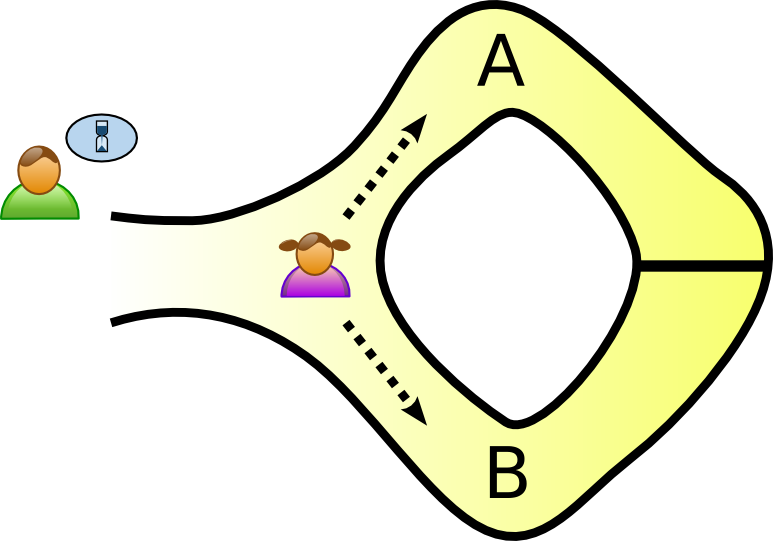
\includegraphics[width=0.44\textwidth]{Figures/Zkip_alibaba1.png}
        \label{fig:bc1}
        \caption{Peggy chooses a path uniformly from $A, B$ without Victor knowing.}
    \end{subfigure}
    \\
    \begin{subfigure}[b]{0.8\textwidth}
    \centering
        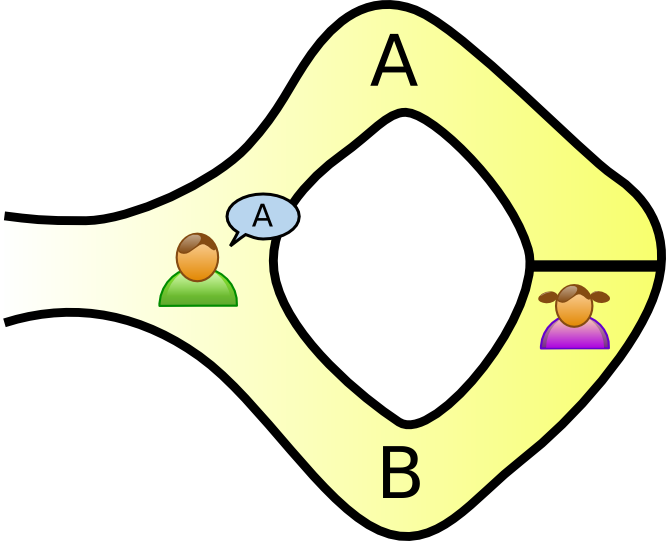
\includegraphics[width=0.4\textwidth]{Figures/Zkip_alibaba2.png}
        \label{fig:bc2}
        \caption{Victor asks her to come out of the cave from path $A$.}
    \end{subfigure}
    \\
    \begin{subfigure}[b]{0.8\textwidth}
    \centering
        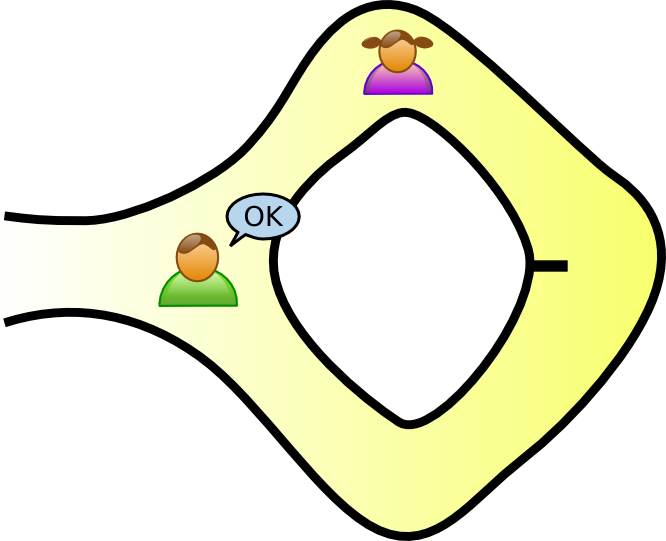
\includegraphics[width=0.4\textwidth]{Figures/Zkip_alibaba3.png}
        \label{fig:bc3}
        \caption{If Peggy had entered from path $A$, she returns trivially. Otherwise, she could open the door using the secret key and return from path $A$.}
    \end{subfigure}
    
    \caption{Example of a zero knowledge proof}
    \label{fig:zkp_alibaba}
    \end{figure}
    
In the above example, Peggy knows the secret word used to open a mysterious door in a cave. The cave is shaped like a horse-hoe. The entrance is on one side and the magic door blocking the opposite side. Victor wants to know whether Peggy knows the secret word; but Peggy, does not want to reveal her knowledge (the secret word) to Victor or to reveal the fact of her knowledge to anyone in the world. 

Peggy and Victor run the protocol described in figure \ref{fig:zkp_alibaba}. Provided she really does know the magic word, and the path she enters and path Victor asks her to come from are same, then it's trivial for Peggy to succeed and Victor to believe that she actually knows the secret key. Further, if the chosen path by Peggy and asked by Victor doesn't match, even then she could open the door and return from a desired path. If they were to repeat this protocol many times, say 15 times in a row, her chance of successfully "guessing" all of Victor's requests would become exponentially small (about three in a lakh).

For zero-knowledge arguments presented in this report, we will consider arguments consisting of three interactive probabilistic polynomial time algorithms $(\text{Setup}, \mathcal{P}, \mathcal{V})$. These algorithms are described by:
\begin{itemize}[label=$\ast$]
    \item Setup: $\sigma \leftarrow \text{Setup}(1^{\lambda})$, $\sigma$ is common reference string
    \item $\mathcal{P}$: prover, $\mathcal{V}$: verifier
    \item Transcript $tr \leftarrow \langle \mathcal{P}, \mathcal{V} \rangle$
    \item $\langle \mathcal{P}, \mathcal{V} \rangle = b$, $b=0$ if the verifier rejects or $b=1$ accepts 
\end{itemize}

Further, we define the relation $\mathcal{R}$ and the CRS-dependent language as:
\begin{align*}
    \mathcal{R} &:= \{ (\sigma, u, w) \in \{0,1\}^{\ast} \times  \{0,1\}^{\ast} \times  \{0,1\}^{\ast}: \ w \ \text{is a witness for}\ u \ | \ \sigma \}\\
    \mathcal{L}_{\sigma} &:=  \{ x \ | \exists w \in (\sigma, u, w) \in \mathcal{R} \}
\end{align*}

So, $\mathcal{L}_{\sigma}$ is essentially the set of statements $x$ that have a witness $w$ in the relation $\mathcal{R}$. 

\subsection{Defining Zero-Knowledge Arguments of Knowledge}
\label{subsec:zka/d_aok}
To mathematically define the notion of zero-knowledge and zero-knowledge arguments, we will provide the necessary definitions below.

\begin{defn}[Argument of Knowledge]
        The triple $(\text{Setup}, \mathcal{P}, \mathcal{V})$ is called an argument of knowledge for relation $\mathcal{R}$ if it is \textcolor{blue}{perfectly complete} and has \textcolor{blue}{computational witness-extended emulation}.
\end{defn}

\begin{defn}[Perfect completeness]
    $(\text{Setup}, \mathcal{P}, \mathcal{V})$ has perfect completeness if for all non-uniform polynomial time adversaries $\mathcal{A}$

    \begin{equation*}
    \Pr 
    \Big[
    \begin{tabular}{c | l}
         \multirow{2}{*}{$(\sigma, u, w) \not \in \mathcal{R} \ or \ 
         \langle \mathcal{P}(\sigma, u, w), \mathcal{V}(\sigma, u) \rangle = 1$}
         & $\sigma \leftarrow \text{Setup}(1^{\lambda})$
         \\
         & 
         $(u, w) \leftarrow \mathcal{A}(\sigma)$
    \end{tabular}
    \Big] 
    = 1
\end{equation*}
\end{defn}

\emph{Perfect completeness} implies that if a statement is actually true, then an honest verifier is convinced with probability $1$ about the truth of the statement by an honest prover.

\begin{defn}[Computational Witness-Extended Emulation]
    $(\text{Setup}, \mathcal{P}, \mathcal{V})$ has witness-extended
    emulation if for all deterministic polynomial time $P^{*}$ there exists an expected polynomial time
    emulator $\mathcal{E}$ such that for all pairs of interactive adversaries $\mathcal{A}_1 , \mathcal{A}_2$ there exists a negligible function
    $\mu (\lambda)$ such that
    
    \begin{multline*}
    \Bigg|
        \Pr
        \Bigg[
        \begin{tabular}{c | l}
             \multirow{3}{*}{$\mathcal{A}_1(tr) = 1$}
             & $\sigma \leftarrow \text{Setup}(1^{\lambda},)$
             \\
             & 
             $(u, s) \leftarrow \mathcal{A}_2(\sigma),$
             \\
             & $tr \leftarrow \langle (\mathcal{P}^{*}(\sigma, u, s), V(u, s) \rangle$
        \end{tabular}
        \Bigg]
        -\\
        \Pr 
        \Bigg[
            \begin{tabular}{l | l}
                \multirow{2}{*}{$\mathcal{A}_1(tr) = 1 \wedge$}
                &
                $\sigma \leftarrow \text{Setup}(1^{\lambda},)$
                \\
                & 
                $(u, s) \leftarrow \mathcal{A}_2(\sigma),$
                \\
                $(tr\ accepted \implies (\sigma, u, w)\in \mathcal{R})$
                &
                $(tr, w) \leftarrow \mathcal{E}^{\mathcal{O}}(\sigma, u)$
           \end{tabular}
           \Bigg]
    \Bigg|
    \leq \mu(\lambda)
    \end{multline*}
    
    where the oracle is given by  $\mathcal{O} = \langle (\mathcal{P}^{*}(\sigma, u, s), V(u, s) \rangle$, and permits rewinding to a specific point and
    resuming with fresh randomness for the verifier from this point onwards. We can also define com-
    putational witness-extended emulation by restricting to non-uniform polynomial time adversaries
    $\mathcal{A}_1$ and $\mathcal{A}_2$.       
    
\end{defn}

\textit{Computational witness-extended emulation} implies that when an adversary produces an argument to convince the verifier with some probability, then we have a corresponding emulator producing identically distributed argument with same probability, but also a witness.

\begin{defn}[Public coin]
    An argument of knowledge  $(\text{Setup}, \mathcal{P}, \mathcal{V})$ is called public coin if all messages sent from the verifier to the prover are chosen uniformly at random and independent of the prover's messages, i.e., the challenges correspond to the verifier's randomness $\rho$.
\end{defn}

\begin{defn}[Zero Knowledge Argument of Knowledge]
    An argument of knowledge $(\text{Setup}, \mathcal{P}, \mathcal{V})$ is zero knowledge if it reveals no information about $w$ apart from what could be deduced from the fact that $(\sigma, u, w) \in \mathcal{R}$.
\end{defn}

An argument of knowledge is zero knowledge if it does not leak information about $w$ apart from what can be deduced from the fact that $(\sigma, u, w) \in \mathcal{R}$. More explicitly, we note that, a zero knowledge argument of knowledge ensures that no \textsf{PPT} adversary (or verifier) can ever recover $w$ given it's relation with $\sigma, u$.

\begin{defn}[Perfect Special Honest-Verifier Zero-Knowledge]
    A public coin argument of knowledge $(\text{Setup}, \mathcal{P}, \mathcal{V})$ is a perfect special honest verifier zero knowledge (SHVZK) argument of knowledge for $\mathcal{R}$ if there exists a probabilistic polynomial time simulator $\mathcal{S}$ such that for all pairs of interactive adversaries $\mathcal{A}_1 , \mathcal{A}_2$
    
    \begin{multline*}
    \Pr
    \Bigg[
    \begin{tabular}{c | l}
        \multirow{3}{*}{$(\sigma, u, w) \in \mathcal{R} \wedge \mathcal{A}_1(tr) = 1$}
         & $\sigma \leftarrow \text{Setup}(1^{\lambda},)$
         \\
         & 
         $(u, w, \rho) \leftarrow \mathcal{A}_2(\sigma),$
         \\
         & $tr \leftarrow \langle (\mathcal{P}(\sigma, u, s), V(\sigma, u; \rho) \rangle$
    \end{tabular}
    \Bigg]
    \\
    =\Pr
    \Bigg[
    \begin{tabular}{c | l}
        \multirow{3}{*}{$(\sigma, u, w) \in \mathcal{R} \wedge \mathcal{A}_1(tr) = 1$}
         & $\sigma \leftarrow \text{Setup}(1^{\lambda},)$
         \\
         & 
         $(u, w, \rho) \leftarrow \mathcal{A}_2(\sigma),$
         \\
         & $tr \leftarrow \mathcal{S}(u, \rho)$
    \end{tabular}
    \Bigg]
    \end{multline*}

\end{defn}

PSHVZK AoK implies that even if an adversary chooses a
distribution over statements and witnesses, it isn't able to
distinguish between simulated transcript and honestly generated
transcript for $u \in \mathcal{L}_{\sigma}$.





\chapter{Literature Survey}
\label{chap:lit}

In this chapter, we briefly discuss the MimbleWimble protocol and Grin, technical details of recently proposed protocols like Improved Inner Product argument, Bulletproofs \cite{Bunz2018} and Omniring \cite{Lai2019} which inspire the design of \RB protocol.
We also describe \R protocol which is the current state-of-the-art proof of reserves protocol for MimbleWimble based cryptocurrencies.
Finally, we will discuss a few limitations of \R which motivated us to design a better proof of reserves protocol.

% IPP
\section{Improved Inner-Product Argument}
\label{sec:iipa}

% \subsection{Building towards Inner-Product Argument}
% \label{subsec:iipa/ov}
We will define Inner-Product argument which is a proof construction for proving to a verifier that the prover knows two vectors which are hidden in a Pedersen commitment and the the inner product of those two vectors is known. 
% We will first provide simpler protocols which are not necessarily zero-knowledge but our ultimate aim remains to give an inner-product protocol which is efficient and zero knowledge.\\

The inputs to the inner-product argument are independent generators $\textbf{g}, \textbf{h} \in \mathbb{G}^n$, $P\in \G$ and a scalar $c \in \Z_q$. $P$ is a binding vector commitment to $\textbf{a}, \textbf{b}$. 
The argument lets the prover convince a verifier that the prover knows two vectors $\textbf{a}, \textbf{b} \in \Z_q^n$ such that 
\begin{equation*}
    P = \textbf{g}^{\textbf{a}} \textbf{h}^{\textbf{b}} \ \wedge \ 
    c = \langle \textbf{a},\textbf{b} \rangle
\end{equation*}
The inner product argument is an efficient proof system for the language:
\begin{align}
    \mathcal{L}_{\textsf{IP}} &=
    \{ ( \underbrace{\textbf{g}, \textbf{h} \in \mathbb{G}^n, P \in \mathbb{G}, c \in \Z_q}_{\textsl{crs}};\
    \underbrace{\textbf{a}, \textbf{b} \in \Z_q^{n}}_{\textsl{wit}}):\
    \underbrace{P = \textbf{g}^{\textbf{a}}\textbf{h}^{\textbf{b}} \wedge c = \langle \textbf{a}, \textbf{b} \rangle}_{\textsl{stmt}} \}
    \label{eq:ipa1}
\end{align}
Here, \textsl{crs, stmt, wit} are common reference string, statement and witness respectively as defined in Section \ref{scn:notation}.
Clearly, the simplest proof system for (\ref{eq:ipa1}) is: $\mathcal{P}$ sends $\mathcal{V}$ $(\textbf{a},\textbf{b}) \in \Z_q^{n}$, requiring to send $2n$ elements to $\mathcal{V}$. We wish to build an efficient proof which requires much less elements to be exchanged. Recall, the communication cost directly affects \textit{efficiency} of a protocol.\\

Note that the witness-CRS relation in (\ref{eq:ipa1}) is essentially an \texttt{AND} of two different relations. To simplify things to start with the inner-product argument,
we propose to design a proof system for the language:
\begin{align}
    \mathcal{L}_{\textsf{IP\_mod}} &= 
        \{ ( \underbrace{\textbf{g}, \textbf{h} \in \mathbb{G}^n, u, P \in \mathbb{G}}_{\textsl{crs}};\
        \underbrace{\textbf{a}, \textbf{b} \in \Z_q^{n}}_{\textsl{wit}}):\
        \underbrace{P = \textbf{g}^{\textbf{a}}\textbf{h}^{\textbf{b}} \cdot u^{\langle \textbf{a}, \textbf{b} \rangle}}_{\textsl{stmt}} \}
        \label{eq:ipa2}
\end{align}
We will first show a protocol or a proof system for language defined in (\ref{eq:ipa2}) and then prove that the same proof system gives a proof system for language in (\ref{eq:ipa1}) with same complexity. 
Define a hash function $H: \Z_{q}^{2n+1} \rightarrow \G$ such that for input vectors $\textbf{a}_1, \textbf{a}_1^{\prime}, \textbf{b}_1, \textbf{b}_1^{\prime} \in \Z_q^{n/2}, c \in \Z_q$
\begin{align}
    H(\textbf{a}_1, \textbf{a}_1^{\prime}, \textbf{b}_1, \textbf{b}_1^{\prime}, c) 
    & :=
    \textbf{g}_{[:n/2]}^{\textbf{a}_1} \cdot 
    \textbf{g}_{[n/2:]}^{\textbf{a}_1^{\prime}}\cdot
    \textbf{h}_{[:n/2]}^{\textbf{b}_1} \cdot 
    \textbf{h}_{[n/2:]}^{\textbf{b}_1^{\prime}}\cdot
    u^c \ \in \mathbb{G}
\end{align}

Further, we notice that in (\ref{eq:ipa2}), we can write $P$ as\blfootnote{We are denoting the first and second halves of a vector $\textbf{a}$ by color coding to simplify visualization, $\textcolor{blue}{\textbf{a}_{[:n^{\prime}]}}$ as the first half and $\textcolor{red}{\textbf{a}_{[n^{\prime}:]}}$ by second half.}: 
\begin{align*}
    n^{\prime}
    &=
    n/2, \ \textbf{a} = (\textcolor{blue}{\textbf{a}_{[:n^{\prime}]}}, \textcolor{red}{\textbf{a}_{[n^{\prime}:]}}),  \ \textbf{b} = (\textcolor{blue}{\textbf{b}_{[:n^{\prime}]}}, \textcolor{red}{\textbf{b}_{[n^{\prime}:]}}),\\
    P 
    &= 
    H(\textcolor{blue}{\textbf{a}_{[:n^{\prime}]}}, \textcolor{red}{\textbf{a}_{[n^{\prime}:]}}, 
    \textcolor{blue}{\textbf{b}_{[:n^{\prime}]}}, \textcolor{red}{\textbf{b}_{[n^{\prime}:]}}, \langle \textbf{a}, \textbf{b} \rangle)
\end{align*}
We also note that $H$ is additively homomorphic in its inputs, i.e
\begin{multline*}
    H(\textbf{a}_1, \textbf{a}_1^{\prime}, \textbf{b}_1, \textbf{b}_1^{\prime}, c_1)\cdot 
    H(\textbf{a}_2, \textbf{a}_2^{\prime}, \textbf{b}_1, \textbf{b}_2^{\prime}, c_2) 
    =\\ 
    \left(\textbf{g}_{[:n/2]}^{\textbf{a}_1} \cdot 
    \textbf{g}_{[n/2:]}^{\textbf{a}_1^{\prime}}\cdot
    \textbf{h}_{[:n/2]}^{\textbf{b}_1} \cdot 
    \textbf{h}_{[n/2:]}^{\textbf{b}_1^{\prime}}\cdot
    u^{c_1}\right)\cdot
    \left(\textbf{g}_{[:n/2]}^{\textbf{a}_2} \cdot 
    \textbf{g}_{[n/2:]}^{\textbf{a}_2^{\prime}}\cdot
    \textbf{h}_{[:n/2]}^{\textbf{b}_2} \cdot 
    \textbf{h}_{[n/2:]}^{\textbf{b}_2^{\prime}}\cdot
    u^{c_2}\right)
\end{multline*}
\begin{align*}
\implies
    H(\textbf{a}_1, \textbf{a}_1^{\prime}, \textbf{b}_1, \textbf{b}_1^{\prime}, c_1) \ \cdot
    &
    H(\textbf{a}_2, \textbf{a}_2^{\prime}, \textbf{b}_1, \textbf{b}_2^{\prime}, c_2)\\ \vspace{10mm}
    &=
    \left(\textbf{g}_{[:n/2]}^{\textbf{a}_1 + \textbf{a}_2} \cdot 
    \textbf{g}_{[n/2:]}^{\textbf{a}_1^{\prime} + \textbf{a}_2^{\prime}}\cdot
    \textbf{h}_{[:n/2]}^{\textbf{b}_1 + \textbf{b}_2} \cdot 
    \textbf{h}_{[n/2:]}^{\textbf{b}_1^{\prime} + \textbf{b}_2^{\prime}}\cdot
    u^{c_1+c_2}\right)\\\vspace{10mm}
    &=
    H(\textbf{a}_1+\textbf{a}_2, \textbf{a}_1^{\prime} + \textbf{a}_2^{\prime}, \textbf{b}_1+\textbf{b}_2, \textbf{b}_1^{\prime} + \textbf{b}_2^{\prime}, c_1+c_2)
\end{align*}
We now describe a protocol for the language $\mathcal{L}_{\textsf{IP\_mod}}$ (\ref{eq:ipa2}) in argument of knowledge \ref{fig:algo1}.


\subsection{Inner-Product Argument}
\label{subsec:iipa/ipa}
%%%%%%%%%%%%%%%%%%%%%%%%%%%%%%%%%%%%%%%%%%%%%%%%%%%%%%

\begin{figure}[h!]
    \caption{Argument of knowledge for $\L_{\textsf{IP\_mod}}$}
    \label{fig:algo1}
\end{figure}
\begin{mdframed}[skipabove=\topsep]
    \begin{itemize}[itemsep=4pt]
        % Setup Phase
        \item[] \textsl{Setup}($\lambda, \mathcal{L}_{\textsf{IP\_mod}}$):
        \\[-5pt]\rule{\textwidth}{0.4pt}\\ 
        Generate following elements randomly from $\G$: $\ \textbf{g} \rgen \G^{n}, \textbf{h} \rgen \G^n, u \rgen \G$
        \\[2pt]
        \textsl{crs} = $(\G, q, \textbf{g}, \textbf{h}, u, P)$, \textsl{wit} = $(\textbf{a}, \textbf{b}) \in \Z_q^n$, \textsl{stmt}: $P = \textbf{g}^\textbf{a} \cdot \textbf{h}^\textbf{b} \cdot u^{\langle \textbf{a},\textbf{b} \rangle}$
        \vspace{2pt}
    
        % Prover
        \item[] $\langle \mathcal{P}(\textsl{crs, stmt, wit}), \mathcal{V}(\textsl{crs, stmt}) \rangle$ :
        \\[-5pt]\rule{\textwidth}{0.4pt}
    
        \vspace{-4pt}
        \item[] $\P$:\vspace{-4pt}
        \begin{enumerate}[itemsep=5pt]
            \item[(i)] $n^{\prime} = n/2$ 
            
            \item[(ii)] $L = H(\textbf{0}^{n^{\prime}}, 
            \textcolor{blue}{\textbf{a}_{[:n^{\prime}]}},
            \textcolor{red}{\textbf{b}_{[n^{\prime}:]}},
            \textbf{0}^{n^{\prime}},
            \langle \textcolor{blue}{\textbf{a}_{[:n^{\prime}]}},
            \textcolor{red}{\textbf{b}_{[n^{\prime}:]}}
            \rangle)$

            \item[(iii)] $R = H(\textcolor{red}{\textbf{a}_{[n^{\prime}:]}},
            \textbf{0}^{n^{\prime}}, 
            \textbf{0}^{n^{\prime}},
            \textcolor{blue}{\textbf{b}_{[n^{\prime}:]}},
            \langle \textcolor{red}{\textbf{a}_{[n^{\prime}:]}},
            \textcolor{blue}{\textbf{b}_{[n^{\prime}:]}}
            \rangle)$
        \end{enumerate}
      
        \item[] $\mathcal{P} \longrightarrow \V$: $L,R \in \G$
    
        \item[] $\mathcal{V}$: $x \rgen \Z_q$, $\mathcal{V} \longrightarrow \P$: $x$
    
        % \item[] $\mathcal{V} \longrightarrow \P$: $w$
    
        \item[] $\P$:
        \begin{enumerate}[itemsep=5pt]
            \item[(i)] $\textbf{a}^{\prime} = x \cdot
            \textcolor{blue}{\textbf{a}_{[:n^{\prime}]}} + x^{-1}\cdot
            \textcolor{red}{\textbf{a}_{[n^{\prime}:]}}$

            \item[(ii)] $\textbf{b}^{\prime} = x^{-1} \cdot
            \textcolor{blue}{\textbf{b}_{[:n^{\prime}]}} + x\cdot
            \textcolor{red}{\textbf{b}_{[n^{\prime}:]}}$
        \end{enumerate}
        
        \item[] $\mathcal{P} \longrightarrow \V$: $\textbf{a}^{\prime}, \textbf{b}^{\prime} \in \Z_q^{n^{\prime}}$
        
        \item[] $\mathcal{V}$: 
        \begin{enumerate}[itemsep=5pt]
            \item[(i)] $P^{\prime} = L^{(x^2)}\cdot P \cdot R^{(x^{-2})}$
    
            \labelText{\item[(ii)]}{label:veq1_ipma}
            $P^{\prime} \stackrel{?}{=} H(x^{-1}\textbf{a}^{\prime}, x\textbf{a}^{\prime},x\textbf{b}^{\prime}, x^{-1}\textbf{b}^{\prime}, 
            \langle \textbf{a}^{\prime}, \textbf{b}^{\prime} \rangle)$ \hfill{\footnotesize \textit{// Verification equation}}
        \end{enumerate}
      
    \end{itemize}
\end{mdframed}

%%%%%%%%%%%%%%%%%%%%%%%%%%%%%%%%%%%%%%%%%%%%%%%%%%%%%%
\vspace{1cm}
The verifier is convinced because indeed the left hand size of the verification equation (\ref{label:veq1_ipma}) by the verifier can be written as:
\begin{multline*}
    L^{x^2}\cdot P \cdot R^{x^{-2}} = H(\textcolor{blue}{\textbf{a}_{[:n^{\prime}]}} 
    + x^{-2}
    \textcolor{red}{\textbf{a}_{[n^{\prime}:]}},
    x^2\textcolor{blue}{\textbf{a}_{[:n^{\prime}]}} 
    +
    \textcolor{red}{\textbf{a}_{[n^{\prime}:]}},\\
    x^2\textcolor{red}{\textbf{b}_{[n^{\prime}:]}} 
    +
    \textcolor{blue}{\textbf{b}_{[:n^{\prime}]}},
    \textcolor{red}{\textbf{b}_{[n^{\prime}:]}} 
    + x^{-2}
    \textcolor{blue}{\textbf{b}_{[:n^{\prime}]}},
    \langle \textbf{a}^{\prime},\textbf{b}^{\prime} \rangle
    )
\end{multline*}
The key features of this approach are listed below.
\begin{enumerate}
    \item This proof system requires sending $n+2$ elements.
        \item To extract a valid witness $\textbf{a}, \textbf{b} \in \Z^n_q$ from a successful prover, we need to rewind the prover three times. After the prover sends $L, R$ we rewind the prover three times to obtain three tuples $(x_i, \textbf{a}_i^{\prime}, \textbf{b}_i^{\prime}) \ \text{for} \ i=1,2,3$ such that for all distinct $x_i$:  
        \begin{equation}
            L^{(x_i^2)}\cdot P \cdot L^{({-x}_i^2)}
            =
            H(x^{-1}\textbf{a}^{\prime}_i, x_i\textbf{a}^{\prime}_i, x_i\textbf{b}^{\prime}, x_i^{-1}\textbf{b}^{\prime}_i, 
            \langle \textbf{a}^{\prime}, \textbf{b}^{\prime}_i \rangle)
        \end{equation}
        
    \item We can now find $\nu_1, \nu_2, \nu_3 \in \Z_q$ such that,
    \begin{equation*}
        \sum_{i=1}^{3}x_i^2 \nu_i=0, \quad 
        \sum_{i=1}^{3}\nu_i = 1, \quad
        \sum_{i=1}^{3}x_i^{-2} \nu_i=0
    \end{equation*}
    
    \item Thus, $\textbf{a}, \textbf{b}$ can be found by computing:
    \begin{align*}
        \textbf{a} &= \sum_{i=1}^{3}(\nu_i \cdot x_i^{-1} \textbf{a}_i^{\prime} \ \| \ \nu_i \cdot x_i^{1} \textbf{a}_i^{\prime}) \in \Z_q^n\\
        \textbf{b} &= \sum_{i=1}^{3}(\nu_i \cdot x_i^{-1} \textbf{b}_i^{\prime} \ \| \ \nu_i \cdot x_i^{1} \textbf{b}_i^{\prime}) \in \Z_q^n
    \end{align*}
        
    \item Can we still improve? Observe that the test in the verification equation (\ref{label:veq1_ipma}) is equivalent to:
    \begin{align*}
    P^{\prime} \stackrel{?}{=} 
    \big(
    \textbf{g}^{x^{-1}}_{[:n^{\prime}]} \circ \textbf{g}^x_{[n^{\prime}:]}
    \big)^{\textbf{a}^{\prime}}
    \cdot
    \big(
    \textbf{h}^x_{[:n^{\prime}]} \circ \textbf{h}^{x^{-1}}_{[n^{\prime}:]}
    \big)^{\textbf{b}^{\prime}}
    \cdot 
    u^{\langle \textbf{a}^{\prime},\textbf{b}^{\prime} \rangle}
    \end{align*}

    \item Thus the prover can recursively engage in an inner-product argument for $P^{\prime}$ with respect to generators:
    \begin{equation*}
        (\textbf{g}^{x^{-1}}_{[:n^{\prime}]} \circ \textbf{g}^x_{[n^{\prime}:]}, \textbf{h}^x_{[:n^{\prime}]} \circ \textbf{h}^{x^{-1}}_{[n^{\prime}:]},u)
    \end{equation*}

    \item We hope to get a total communication of Protocol 2 to be only $2\lceil \text{log}_2 (n) \rceil$ elements in $\mathbb{G}$ plus 2 elements in $\Z_q$. Let's see how we go about doing it in the next section.
    
\end{enumerate}


\subsection{Recursive Inner-Product Argument}
\label{subsec:iipa/recursion}

\begin{figure}[h!]
    \caption{Improved Inner-Product Argument for $\L_{\textsf{IP\_mod}}$}
    \label{algo2}
\end{figure}
\begin{mdframed}[skipabove=\topsep]
    \begin{itemize}[itemsep=4pt]
        % Setup Phase
        \item[] \textsl{Setup}($\lambda, \mathcal{L}_{\textsf{IP\_mod}}$):
        \\[-5pt]\rule{\textwidth}{0.4pt}\\ 
        Generate following elements randomly from $\G$: $\ \textbf{g} \rgen \G^{n}, \textbf{h} \rgen \G^n, u \rgen \G$
        \\[2pt]
        \textsl{crs} = $(\G, q, \textbf{g}, \textbf{h}, u, P)$, \textsl{wit} = $(\textbf{a}, \textbf{b}) \in \Z_q^n$, \textsl{stmt}: $P = \textbf{g}^\textbf{a} \cdot \textbf{h}^\textbf{b} \cdot u^{\langle \textbf{a},\textbf{b} \rangle}$
        \vspace{2pt}
    
        % Prover
        \item[] $\langle \mathcal{P}(\textsl{crs, stmt, wit}), \mathcal{V}(\textsl{crs, stmt}) \rangle$ :
        \\[-5pt]\rule{\textwidth}{0.4pt}

        \vspace{-4pt}
        \item[] $\P$: If $n^{\prime} = 1$: \vspace{-4pt}
        
        \item[] $\mathcal{P} \longrightarrow \V$: $a,b \in \Z_q$
        
        \vspace{-4pt}
        \item[] $\mathcal{V}$: \vspace{-4pt}
        \begin{enumerate}[itemsep=5pt]
            \item[(i)] $c = a \cdot b$
    
            \labelText{\item[(ii)]}{label:veq1_iipa}
            $P \stackrel{?}{=} g^a h^b u^c$ \hfill{\footnotesize \textit{// Single exponentiation verification equation}}
        \end{enumerate}
    
        \vspace{-4pt}
        \item[] $\P$: Else $n^{\prime} > 1$: \vspace{-4pt}
        \begin{enumerate}[itemsep=5pt]
            \item[(i)] $n^{\prime} = n/2$ where $n = |\textbf{g}|$ 
            
            \item[(ii)] $c_L = \langle \textcolor{blue}{\textbf{a}_{[:n^{\prime}]}},
            \textcolor{red}{\textbf{b}_{[n^{\prime}:]}}
            \rangle \in \Z_q$, 

            \item[(iii)] $c_R = \langle \textcolor{red}{\textbf{a}_{[n^{\prime}:]}},
            \textcolor{blue}{\textbf{b}_{[n^{\prime}:]}}
            \rangle \in \Z_q$

            \item[(iv)] $L = \textbf{g}^{\textcolor{blue}{\textbf{a}_{[:n^{\prime}]}}}_{[n^{\prime}:]} 
            \cdot \textbf{h}^{\textcolor{red}{\textbf{b}_{[n^{\prime}:]}}}_{[:n^{\prime}]} \cdot u^{c_L} \in \mathbb{G}$
 
            \item[(v)] $R = \textbf{g}^{\textcolor{red}{\textbf{a}_{[n^{\prime}:]}}}_{[:n^{\prime}]} 
            \cdot \textbf{h}^{\textcolor{blue}{\textbf{b}_{[n^{\prime}:]}}}_{[n^{\prime}:]} \cdot u^{c_R} \in \mathbb{G}$
        \end{enumerate}
      
        \item[] $\mathcal{P} \longrightarrow \V$: $L,R \in \G$
    
        \item[] $\mathcal{V}$: $x \rgen \Z_q$, $\mathcal{V} \longrightarrow \P$: $x$
    
        % \item[] $\mathcal{V} \longrightarrow \P$: $w$

        \item[] $\P, \ \V$:
        \begin{enumerate}[itemsep=5pt]
            \item[(i)] $\textbf{g}^{\prime} = \textbf{g}^{x^{-1}}_{[:n^{\prime}]} \circ \textbf{g}^x_{[n^{\prime}:]} \in \mathbb{G}^{\prime}$

            \item[(ii)] $\textbf{h}^{\prime} = \textbf{h}^x_{[:n^{\prime}]} \circ \textbf{h}^{x^{-1}}_{[n^{\prime}:]} \in \mathbb{G}^{\prime}$

            \item[(iii)] $P^{\prime} = L^{x^2}PR^{x^{-2}} \in \mathbb{G}$
        \end{enumerate}
    
        \item[] $\P$:
        \begin{enumerate}[itemsep=5pt]
            \item[(i)] $\textbf{a}^{\prime} = x \cdot
            \textcolor{blue}{\textbf{a}_{[:n^{\prime}]}} + x^{-1}\cdot
            \textcolor{red}{\textbf{a}_{[n^{\prime}:]}}
            \in \Z^{n^{\prime}}_q$

            \item[(ii)] $\textbf{b}^{\prime} = x^{-1} \cdot
            \textcolor{blue}{\textbf{b}_{[:n^{\prime}]}} + x\cdot
            \textcolor{red}{\textbf{b}_{[n^{\prime}:]}}
            \in \Z^{n^{\prime}}_q$
        \end{enumerate}

        \item[] Set \textsl{crs'} = $(\G, q, \textbf{g}^{\prime}, \textbf{h}^{\prime}, u, P^{\prime})$, \textsl{wit'} = $(\textbf{a}^{\prime}, \textbf{b}^{\prime}) \in \Z_q^n$, \textsl{stmt'}: $P^{\prime} = (\textbf{g}^{\prime})^{\textbf{a}^{\prime}} \cdot (\textbf{h}^{\prime})^{\textbf{b}^{\prime}} \cdot u^{\langle \textbf{a}^{\prime},\textbf{b}^{\prime} \rangle}$
      
        \item[] Run Protocol \ref{algo2} with $\langle \mathcal{P}(\textsl{crs', stmt', wit'}), \mathcal{V}(\textsl{crs', stmt'}) \rangle$  \hfill{\footnotesize \textit{// Recursion step}}
      
    \end{itemize}
\end{mdframed}

In the above recursive inner-product protocol, the resulting depth is of the order of $ \text{log}_2(n)$. The total communication in this protocol is $2 \times \lceil \text{log}_2(n) \rceil$ elements in $\G$ and $2$ elements in $\Z_q$, i.e the prover sends the following in the specified order:
\begin{equation*}
    (L_1, R_1), \dots, (L_{\text{log}_2(n)}, R_{\text{log}_2(n)}), a, b
\end{equation*}
Now, coming back to the language defined in (\ref{eq:ipa1}), we now are in an position to design a proof system for (\ref{eq:ipa1}). 
The improved inner product protocol for the relation (\ref{eq:ipa1}) is presented in Figure \ref{algo3}.
\vspace{0.2cm}

\begin{figure}[h!]
    \caption{Improved Inner-Product Argument for $\L_{\textsf{IP}}$ (\ref{eq:ipa1}) }
    \label{algo3}
\end{figure}
\begin{mdframed}
    \begin{itemize}[itemsep=4pt]
        % Setup Phase
        \item[] \textsl{Setup}($\lambda, \mathcal{L}_{\textsf{IP}}$):
        \\[-5pt]\rule{\textwidth}{0.4pt}\\ 
        Generate following elements randomly from $\G$: $\ \textbf{g} \rgen \G^{n}, \textbf{h} \rgen \G^n, u \rgen \G$
        \\[2pt]
        \textsl{crs} = $(\G, q, \textbf{g}, \textbf{h}, u, P)$, \textsl{wit} = $(\textbf{a}, \textbf{b}) \in \Z_q^n$, \textsl{stmt}: $P = \textbf{g}^\textbf{a} \cdot \textbf{h}^\textbf{b} \cdot u^{\langle \textbf{a},\textbf{b} \rangle}$
        \vspace{2pt}
    
        % Prover
        \item[] $\langle \mathcal{P}(\textsl{crs, stmt, wit}), \mathcal{V}(\textsl{crs, stmt}) \rangle$ :
        \\[-5pt]\rule{\textwidth}{0.4pt}

        \vspace{-4pt}
        \item[] $\mathcal{V}$: $x \rgen \Z_q$, $\mathcal{V} \longrightarrow \P$: $x$
    
        \vspace{-4pt}
        \item[] $\P$: \vspace{-4pt}
        \begin{enumerate}[itemsep=5pt]
            \item[(i)] $P^{\prime} = P \cdot U^{x \cdot c}$ 
        \end{enumerate}

        \item[] Set \textsl{crs'} = $(\G, q, \textbf{g}, \textbf{h}, u^x, P^{\prime})$, \textsl{wit'} = $(\textbf{a}, \textbf{b}) \in \Z_q^n$
      
        \item[] Run Protocol \ref{algo2} with $\langle \mathcal{P}(\textsl{crs', stmt, wit'}), \mathcal{V}(\textsl{crs', stmt}) \rangle$
      
    \end{itemize}
\end{mdframed}

Therefore, the above is the improved inner product argument for the language defined in (\ref{eq:ipa1}).
We now state the Inner-Product Argument which shows that Protocol \ref{algo3} is a proof system for (\ref{eq:ipa1}).

\begin{theorem}[Improved Inner-Product Argument]
    The argument presented in Figure \ref{algo3} for the relation (\ref{eq:ipa1}) has perfect completeness and statistical witness-extended-emulation for either extracting a non-trivial discrete logarithm relation between $\textbf{g}, \textbf{h}, u$ or extracting a valid witness $\textbf{a}, \textbf{b}$.
\end{theorem}
\textit{Proof:} The proof for above theorem is given in Appendix B in \cite{Bunz2018}.


% Bulletproofs
\section{Bulletproofs}
\label{sec:bulletproofs}

Bulletproofs \cite{Bunz2018} is the state-of-art range proof with logarithmic communication size.
A range proof is a zero-knowledge proof showing that a given number lies in a particular range without revealing the number itself.
In this section, we review the logarithmic range proof protocol presented in Bulletproofs paper.

We wish to design a proof system for the following relation which is equivalent to the range proof language
\begin{align}
    \mathcal{L}_{\textsf{BP}} &= \big\{ (\underbrace{g,h, V \in \mathbb{G}, \ n \in \N}_{\textsl{crs}}; \ \underbrace{v, \gamma \in \Z_q}_{\textsl{wit}}): \ \underbrace{V = g^v h^{\gamma} \wedge v \in [0, 2^n)}_{\textsl{stmt}} \big\}
    \label{eqn:lang_bp}
\end{align}

Let $\textbf{a}_L = (a_1, \dots, a_n) \in \{0,1\}^n$ be the vector containing the bits of $v$, $v = \langle \textbf{a}_L,\textbf{2}^n \rangle$. 
Recall that $\textbf{2}^n = (1, 2^1, 2^2, \dots, 2^{n-1}) \in \Z_q^n$.
Prover $\mathcal{P}$ convinces the verifier that $v \in [0,2^n -1]$ by proving that:
\begin{enumerate}
    \item It knows $\textbf{a}_L \in \Z_q^{n}, \ v, \gamma \in \Z_q$ such that $V=g^vh^{\gamma}$
    \item $\langle \textbf{a}_L,\textbf{2}^n \rangle =v
    \ \text{and } \  \textbf{a}_L \circ \textbf{a}_R = \textbf{0}^n \ \text{and } \ 
    \textbf{a}_R = \textbf{a}_L - \textbf{1}^n$
\end{enumerate}

To do so, we take a random linear combination (chosen by the verifier) of the constraints to use inner-product argument. Note that $\langle \textbf{b},\textbf{y}^n \rangle = 0, y \in \Z_q \implies \textbf{b} = \textbf{0}^n$. For randomly chosen $y, z \in \Z_q$, we can write: 
\begin{align}
    z^2 \cdot \langle \textbf{a}_L,\textbf{2}^n \rangle +
    z \cdot \langle \textbf{a}_L - \textbf{1}^n - \textbf{a}_R,\textbf{y}^n \rangle +
    \langle \textbf{a}_L,\textbf{a}_R \circ \textbf{y}^n \rangle =
    z^2 \cdot v
\end{align}
\begin{align}
    \implies \
    \big\langle
    \underbrace{\textbf{a}_L - z\cdot \textbf{1}^n}_{\textsl{left secret}}, \
    \underbrace{\textbf{y}^n \circ (\textbf{a}_R + z\cdot \textbf{1}^n) + z^2 \cdot \textbf{2}^n}_{\textsl{right secret}}
    \big\rangle
    =
    z^2 + \delta(y,z)
    \label{iprf1}
\end{align}
\vspace{-5mm}
\begin{align*}
    \delta(y, z) 
    =
    (z-z^2)\cdot \langle \textbf{1}^n,\textbf{y}^n \rangle - z^3\langle \textbf{1}^n,\textbf{2}^n \rangle
\end{align*}

Here, $\delta(y,z) \in \Z_q$ is a quantity that the verifier can easily calculate since $y,z \in \Z_q^{\star}$ are the challenges generated by the verifier himself. So now, if the prover could send to the verifier the two vectors in the inner product in (\ref{iprf1}), then the verifier could check (\ref{iprf1}) using the commitment $V$ to $v$. Thus the verifier would be convinced that $v \in [0, 2^n-1]$. But there's an issue in this approach. The verifier can easily extract $\textbf{a}_L$ from the first vector which the prover sent for calculation of inner product. 

To address this issue, by introducing two additional blinding terms $\textbf{s}_L, \textbf{s}_R \in \Z_q^{n}$ to blind these vectors. Thus, we define two linear vector polynomials\\
$l(X), r(X) \in \Z_q^n [X]$ and $t(X) \in \Z_q$ as follows:
\vspace{-4mm}
\begin{align*}
    l(X) &= \textbf{a}_L - z\cdot \textbf{1}^n + \textbf{s}_L \cdot X\\
    r(X) &= \textbf{y}^n \circ (\textbf{a}_R + z\cdot \textbf{1}^n + \textbf{s}_R\cdot X) + z^2 \cdot \textbf{2}^n\\
    t(X) &= \langle l(X),r(X) \rangle = t_0 + t_1 \cdot X + t_2 \cdot X^2
    \intertext{where}
    t_0 &= \big\langle
    \textbf{a}_L - z\cdot \textbf{1}^n, \
    \textbf{y}^n \circ (\textbf{a}_R + z\cdot \textbf{1}^n) + z^2 \cdot \textbf{2}^n
    \big\rangle\\
    t_1 &= \big\langle
    \textbf{a}_L - z\cdot \textbf{1}^n, \textbf{y}^n \circ \textbf{s}_R  
    \big\rangle
    +
    \big\langle
    \textbf{s}_L, \left( \textbf{y}^n \circ (\textbf{a}_R + z\cdot \textbf{1}^n) + z^2 \cdot \textbf{2}^n \right)
    \big\rangle
    \\
    t_2 &= \big\langle
    \textbf{s}_L, \textbf{y}^n \circ \textbf{s}_R
    \big\rangle
\end{align*}

The constant term of $\langle l(X),r(X) \rangle$ are the required inner product vectors in (\ref{iprf1}). Now, the prover can publish  $l(x)$ and $r(x)$ for one $x \in \Z_q$. 
The constant term of $t(X)$, denoted $t_0$, is the result of the inner product. The prover needs to convince the verifier that this $t_0$ satisfies $t_0 = z^2\cdot v + \delta(y,z)$. 
To so do, the prover commits to the remaining coefficients of $t(X)$, $t_1, t_2 \in \Z_q$.

\begin{figure}[h!]
\caption{Inner Product Range Proof for $\L_{\textsf{BP}}$}
\label{fig:protocol_BP}
\end{figure}
\vspace{-12pt}
\begin{mdframed}
\begin{itemize}[itemsep=4pt]
    % Setup Phase
    \item[] \textsl{Setup}($\lambda, \L_{\textsf{BP}}$):
    \\[-5pt]\rule{\textwidth}{0.4pt}\\ 
    Generate following elements randomly from $\G$: $h \rgen \G, \ \textbf{g}, \textbf{h} \rgen \G^{n}$
    \\[2pt]
    Set: (\textsl{crs, stmt, wit}) as defined in the language $\L_{\textsf{BP}}(\G, q, \textbf{g}, \textbf{h}, h)$ in (\ref{eqn:lang_bp})
    \vspace{2pt}

    % Prover
    \item[] $\langle \mathcal{P}(\textsl{crs, stmt, wit}), \mathcal{V}(\textsl{crs, stmt}) \rangle$ :
    \\[-5pt]\rule{\textwidth}{0.4pt}

    % \item[] $\mathcal{V}$: $u,v \rgen \Z$, $\mathcal{V} \longrightarrow \P$: $u, v$

    % \item[] $\mathcal{V} \longrightarrow \P$: $u$
    
    % \item[] $\P, \ \V$:
    % \begin{enumerate}[itemsep=5pt]
    %     \item[(i)] $\hat{I} \coloneqq \ \textbf{I}^{- \vecnb{u}^s}$
        
    %     \item[(ii)] For $w \in \Z_q$, write
    %     \vspace{-4pt}
    %     \begin{equation}
    %       \textbf{g}_{w} \coloneqq \big[ \big((g \| g_t \| \textbf{C} \| \hat{I})^{\circ w} \circ \textbf{p}\big) \|\textbf{g}^{\prime} \big]
    %     \end{equation}
    % \end{enumerate}

    \vspace{-4pt}
    \item[] $\P$:\vspace{-4pt}
    \begin{enumerate}[itemsep=5pt]
        \item[(i)] Set $\textbf{a}_L \in \{0,1\}^n$ such that $\textbf{a}_L, \textbf{2}^n = v$
        \item[(ii)] Set $\textbf{a}_R = \textbf{a}_L - \textbf{1}^n \in \mathbb{Z}_q^n$
        \item[(iii)] $\alpha \leftarrow \mathbb{Z}_q$ 
        \item[(iv)] $A = h^{\alpha}\textbf{g}^{\textbf{a}_L}\textbf{h}^{\textbf{a}_R}$
        \item[(v)] $\textbf{s}_L, \textbf{s}_R \leftarrow \mathbb{Z}_q^n$
        \item[(vi)] $\rho \leftarrow \mathbb{Z}_q$
        \item[(vii)] $S = h^{\rho}\textbf{g}^{\textbf{s}_L}\textbf{h}^{\textbf{s}_R}$ 
        \item[(viii)] $\tau_1, \tau_2 \leftarrow \mathbb{Z}_q$
        \item[(ix)] $T_i = g^{t_i}h^{\tau_i}$, $i \in \{ 1,2\}$ 
    \end{enumerate}

    \item[] $\mathcal{P} \longrightarrow \V$: $A, S, T_1, T_2 \in \G$ 

    \item[] $\mathcal{V}$: $x,y,z \rgen \Z_q$, $\mathcal{V} \longrightarrow \P$: $x,y,z$

    % \item[] $\mathcal{V} \longrightarrow \P$: $w$

    \item[] $\P$:\vspace{-4pt}
    \begin{enumerate}[itemsep=5pt]
        \item[(i)] $\textbf{l} = l(x) = \textbf{a}_L - z\cdot \textbf{1}^n + \textbf{s}_L \cdot x \ \in \mathbb{Z}_q^n$
        \item[(ii)] $\textbf{r} = r(x) = \textbf{y}^n \circ (\textbf{a}_R + z\cdot \textbf{1}^n + \textbf{s}_R\cdot X) + z^2 \cdot \textbf{2}^n \ \in \mathbb{Z}_q^n$
        \item[(iii)] $\hat{t} = \langle \textbf{l}, \textbf{r}\rangle \in \mathbb{Z}_q$
        \item[(iv)] $\tau_x = \tau_2\cdot x^2 + \tau_1\cdot x + z^2\cdot \gamma \in \mathbb{Z}_q$
        \item[(v)] $\mu = \alpha + \rho \cdot x \in \mathbb{Z}_q$
    \end{enumerate}

    \item[] $\mathcal{P} \longrightarrow \V$: $ \textbf{l},\textbf{r} \in \Z_q^n, \ \tau_x, \mu, \hat{t} \in \Z_q$
    
    \item[] $\mathcal{V}$: 
    \begin{enumerate}[itemsep=5pt]
        \item[i] $h^{\prime}_i = h_i^{(y^{-i+1})} \in \mathbb{G}, \forall i$
        \item[(ii)] $P = A\cdot S^x \cdot \textbf{g}^{-z} \cdot
        (\textbf{h}^{\prime})^{z\cdot \textbf{y}^n + z^2 \cdot \textbf{2}^n} \in \mathbb{G}$
          
        \labelText{\item[(iii)]}{label:veq1_bp}
        $\hat{t} \stackrel{?}{=}
        \langle \textbf{l},\textbf{r}\rangle \in \mathbb{Z}_q$
        \hfill{{\small \textit{// $\hat{t}$ was computed correctly}}}

        \labelText{\item[(iv)]}{label:veq2_bp}
        $ g^{\hat{t}}
        h^{\tau_x} 
        \stackrel{?}{=}
        V^{z^2} 
        \cdot
        g^{\delta(y,z)} 
        \cdot 
        T_1^{x} 
        \cdot 
        T_2^{x^2}$
        \hfill{{\small \textit{// $\hat{t}$ satisfies $t_0 + t_1x + t_2x^2$}}} 

        \labelText{\item[(v)]}{label:veq3_bp}
        $P \stackrel{?}{=}
        h^{\mu} \cdot \textbf{g}^{\textbf{l}} \cdot (\textbf{h}^{\prime})^{\textbf{r}}$
        \hfill{{\small \textit{// Check if $\lvec = l(x)$ and $\rvec = r(x)$}}}
        
    \end{enumerate}
\end{itemize}
\end{mdframed}
Some key observations from the above protocol in Figure \ref{fig:protocol_BP} are:
\begin{enumerate}
    \item In this protocol, $\mathcal{P}$ sends $(\textbf{l}, \textbf{r})$, whose size is linear in $n$.
    \item The total communication cost in this protocol is $2n+4$ elements in $\mathbb{G}$ and $3$ elements in $\mathbb{Z}_q$.
    \item The verifier, to check if the received $\textbf{l}, \textbf{r}$ are actually $l(x), r(x)$ and also check if $t(x)=\langle \textbf{l}, \textbf{r}\rangle$, first, switches the generators of the commitment from $\textbf{h} \in \mathbb{G}^n$ to $\textbf{h}^{\prime} = \textbf{h}^{(\textbf{y}^{-n})}$.   
    \item Now, $A$ becomes a Pedersen vector commitment to $(\textbf{a}_L, \textbf{a}_R \circ \textbf{y}^n)$ w.r.t $(\textbf{g}, \textbf{h}^{\prime}, h)$. Similarly, $S$ is now a Pedersen vector commitment to $(\textbf{s}_L, \textbf{s}_R \circ \textbf{y}^n)$.
    \item If all three conditions marked by red rectangle result in a positive answer to the verifier, (s)he accepts and thus prover succeeds.
\end{enumerate}

\begin{theorem}[Range Proof]
    The range proof presented above has perfect completeness, perfect special honest verifier zero-knowledge, and computational witness extended emulation.
    \label{thm:rp}
\end{theorem}
\textit{Proof:} The range proof is a special case of the aggregated range proof with $m=1$. Refer Appendix C in \cite{Bunz2018} for the proof of the theorem \ref{thm:rp}.

In the above protocol, prover had to transfer $\textbf{l} \in \Z_q^n$ and $\textbf{r} \in \Z_q^n$ resulting in proof size proporional to $2n$. 
For a proof whose size is logarithmic in $n$, we can eliminate the transfer of $\textbf{l}$ and $\textbf{r}$ using the inner-product argument. 
We also observe that vectors $(\textbf{l}, \textbf{r})$ are not secret and hence a protocol that only provides soundness\footnote{\textit{Soundness} is the property of only being able to prove "true" things. \textit{Completeness} is the property of being able to prove all true things. \cite{sc13}} is sufficient. 

Concretely, observe that verifying first and third checks of the protocol in Figure \ref{fig:protocol_BP} is the same as verifying that the witness $(\textbf{l}, \textbf{r})$ satisfies the inner product relation (\ref{eq:ipa1}) on public input $(\textbf{g}, \textbf{h}^{\prime}, Ph^{-\mu}, \hat{t})$, where $P$ is a Pedersen vector commitment to vectors $\textbf{l}, \textbf{r} \in \mathbb{Z}_q^n$ whose inner product is $\hat{t}$.
\vspace{-2mm}
\begin{align*}
        P & \stackrel{?}{=}  h^{\mu} \cdot \textbf{g}^{\textbf{l}} \cdot (\textbf{h}^{\prime})^{\textbf{r}}
        \\
        \hat{t} & \stackrel{?}{=} \langle \textbf{l},\textbf{r}\rangle \in \mathbb{Z}_q
        \\
        \vspace{2mm}
        \{ (\textbf{g}, \textbf{h} \in \mathbb{G}^n, P \in \mathbb{G}, c \in & \mathbb{Z}_q ;\ 
        \textbf{a}, \textbf{b} \in \mathbb{Z}_q^{n}) :\
        P = \textbf{g}^{\textbf{a}}\textbf{h}^{\textbf{b}} \wedge c = \langle \textbf{a}, \textbf{b} \rangle \}
    \end{align*}
    
Thus, using the inner product argument, the total communication cost reduces down to $\textcolor{black}{2\lceil \text{log}_2(n) \rceil + 4}$ elements in $\mathbb{G}$ and $\textcolor{black}{5}$ elements in $\mathbb{Z}_q$.


% Omniring
\section{Omniring}
\label{scn:omniring}

Omniring \cite{Lai2019} was proposed as a novel RingCT scheme which (i) did not require any trusted setup,
(ii) had a proof size logarithmic in the size of the ring, and (iii) allowed to share the same
ring between all source addressed in a transaction, thereby enabling significantly improved privacy.
Omniring provides key insights in the direction of generalising Bulletproofs \cite{Bunz2018} framework for RingCT applications.

\subsection{Main Idea}
\label{subscn:idea_omniring}

We start with a ring $\mathcal{R} = (P_1, P_2, \dots, P_n) \in \G^n$ of public keys of the form $P_i = g^{x_i}$ where $g \in \G$ is the group generator and $x_i \in \Z_q$ is the secret key, for all $i \in [n]$.
Suppose we own the public keys (addresses) at indices $(i_1, i_2, \dots, i_s)$ such that each $i_j \in [n]$ for all $j \in [s]$ and $s < n$.
This implies that we know the secret keys $\textbf{x} = (x_{i_1}, x_{i_2}, \dots, x_{i_s})$.
We would like to prove the knowledge of tuples $(i_j, x_{i_j})$ for $j \in [s]$.
For all $j\in [s]$, let us define unit vectors $\textbf{e}_{j} \in \{0,1\}^n$ such that it has $1$ only in position $i_j$.
Therefore,
\begin{align}
    1 &= g^{-x_j} \mathcal{R}^{\textbf{e}_{j}} \text{ for all } j \in [s]. \nonumber \\
    \intertext{Combining the above equations using powers of a scalar challenge $u \in \Z_q$, we get}
    \implies 1 &= g^{- \langle \vecnb{u}^s, \textbf{x} \rangle} \cdot \mathcal{R}^{\sum_{j=1}^s u^{j-1} \textbf{e}_{j}}.
    \label{eqn:maineq_omniring}
\end{align}
We will refer to equation (\ref{eqn:maineq_omniring}) as the \textit{main equality}.
By embedding the bases $(g \| \mathcal{R})$ and secrets $\textbf{a} = (\textbf{e}_{1}, \textbf{e}_2, \dots, \textbf{e}_s, x_{i_1}, x_{i_2}, \dots, x_{i_s})$ in the main equality in form of a Pedersen vector commitment, we can build an inner product relationship between the secrets and challenges to use the Bulletproofs framework in building a RingCT.
However, the soundness of Bulletproofs is guaranteed because the elements in the base vectors used in the Pedersen vector commitment are independent and uniformly random.
In this case, the prover might know the discrete log relationship between some elements in $\mathcal{R}$ since he owns multiple addresses.
To overcome this, Lai et al. \cite{Lai2019} proposed using base vector of the form:
\begin{equation*}
    \textbf{g}_w \coloneqq (g \| \mathcal{R})^{\circ w} \circ \textbf{p},
\end{equation*}
where $w \in \Z_q$ and $\textbf{p} \rgen \G^{n+1}$. 
A \textsf{PPT} adversary cannot find the discrete log relation between the elements of the newly constructed base $\textbf{g}_w$ (refer to Lemma \ref{thmNoDLBase}).
Note that $\textbf{g}_w^{\textbf{a}} = \textbf{g}_{w^{\prime}}^{\textbf{a}}$ for any $w, w^{\prime} \in \Z_q$ because of the main equality.
Therefore, using the new base vector for two different challenges $w, w^{\prime} \in \Z_q$, we can run a Bulletproofs-like protocol twice and extract the secret vectors.
This ensures that the Bulletproofs-like protocol preserves soundness.





% Grin overview
\section{Overview of MimbleWimble \& Grin}
\label{scn:grin_overview}

MimbleWimble \cite{Poelstra2016} is a blockchain protocol relying only on elliptic curve cryptography and promises to provide scalability, privacy and fungibility all at once.
Interestingly, MimbleWimble does not have any addresses or accounts and the amounts also are hidden using Pedersen commitments.
The simple design of MimbleWimble coupled with its privacy and scalability guarantees (which most existing blockchain implementations fail to address collectively) is what makes it popular for use in decentralized systems.
Grin \cite{GrinWebsite} and Beam \cite{BeamWebsite} are cryptocurrency systems which are powered by the MimbleWimble protocol.

\subsection{Outputs in Grin}

Amounts in MimbleWimble are hidden in Pedersen commitments known as \textit{outputs}.
An output containing amount $a \in \{0,1,\dots, 2^{64}-1\}$ is of the form\footnote{We use additive notation in this section only to be consistent with the original MimbleWimble protocol in \cite{Poelstra2016}.} $P = kG + aH$ where $r \in \Z_q$ and $G,H$ are generators of $\G$.
Note that the discrete log relation between $G$ and $H$ is assumed to be unknown.
The quantity $k$ is called as the \textit{blinding factor} and it serves as the secret key of output $P$.
Knowledge of $k$ implies ownership of the output.
At the time of creation of new outputs, they are accompanied by a range proof which proves that the amounts hidden in them lie in a finite range.

\subsection{Transactions in Grin}
A Grin transaction consists of some inputs which are being spent and some outputs in which the funds would be deposited.
Note that the inputs in a transaction are essentially outputs which were generated in some block in the past.
Grin transactions are of two types: (i) coinbase transactions, which transfer the block mining rewards to miners and (ii) regular transactions, which makes up for amount transfers in non-miners.
Coinbase transactions do not contain any inputs and typically have just one output known as \textit{coinbase} output.
A regular Mimblewimble transaction \cite{GrinDocOnGithub} includes the following:
\begin{enumerate}
    \item[(i)] A set of inputs, that reference and spend a set of previous outputs,
    \item[(ii)] A set of new outputs each with a range proof,
    \item[(iii)] An transaction fee,
    \item[(iv)] A Schnorr signature whose private key is computed by taking the excess amount (the sum of all output amounts plus the fee, minus the input amounts),
    \item[(v)] The public key published with the Schnorr signature is known as \textit{kernel excess} and is of the form $rG, \ r \in \Z_q$.
\end{enumerate}
We will refer to the collection of transaction fee, public key and signature as a \textit{kernel}.
Note that a transaction can easily be validated by determining that the kernel excess is a valid public key. 

\subsection{Transaction Aggregation}
Transactions in a Grin block are aggregated before the block is added to the blockchain to ensure unlinkability in inputs and outputs.
Consider the following example where we intend to aggregate two given regular transactions.
\begin{table}[h!]
  \centering
    \begin{tabular}{ | m{3cm} | m{2cm}| m{2cm} | m{2cm} | m{2cm} |} 
    \hline
                           & Inputs & Outputs & Excesses & Fee \\
    \hline
    Tx\#1         & $I_1, I_2$ & $O_1$ & $K_1$  & $f_1$ \\ 
    \hline
    Tx\#2         & $I_3$ & $O_2$ & $K_2$  & $f_2$ \\ 
    \hline
    \hline
    Aggregated Tx & $I_1, I_2, I_3$ & $O_1, O_2$ & $K_1, K_2$  & $f_1 + f_2$\\ 
    \hline
    \end{tabular}
  \caption{Example of Transaction Aggregation}
  \label{table:tx_agg}
\end{table}

\noindent
However, there is a slight issue here. 
It is possible to try all combinations of inputs and outputs to recover one of the transactions where the equality 
$$\sum (\text{Ouputs}) + \sum (\text{Fees})H - \sum (\text{Inputs}) = \text{Kernel excess}$$
satisfies. To mitigate this, the kernel excess is redefined from $rG$ to $(r-k_{\text{offset}})G$ where $r$ is the sum of output amounts plus fees minus input amounts and $k_{\text{offset}}$ is a scalar in $Z_q$.
Thus, The kernel offset $k_{\text{offset}}$ is thus a blinding factor that needs to be added to the excess value to ensure the commitments sum to zero as:
\begin{equation*}
  \sum (\text{Ouputs}) + \sum (\text{Fees})H - \sum (\text{Inputs}) = \text{Kernel excess} + k_{\text{offset}}G
\end{equation*}

Further, if in a same block, some outputs generated in a transaction are spent in the same block in another transaction, we can drain those outputs and inputs from the block as the structure of each transaction does not actually matter.
As long as the sum of inputs and outputs cancels off, removing matching outputs would not matter. 
This is known as \textit{cut-through}. 

Going a step further, all the blocks on the Grin blockchain can be considered as individual transactions. 
Thus, the outputs generated at block height $h_1$ which are spent as inputs in block $h_2$ also could be removed from the blockchain as they can be considered intermediate transactions by the same logic as above.
This significantly improves scalability of MimbleWimble-based blockchains.  

\subsection{Grin Blocks}
\label{scn:GrinOverview}

%Grin is an implementation of the MimbleWimble protocol and thus it does not have any addresses.
Let $\mathbb{G}$ be the secp256k1 elliptic curve group of order $n$.
In Grin, coins are stored in Pedersen commitments of the form $C = kG + aH$ where $k, a \in \mathbb{F}_n$ are scalars and $G, H \in \mathbb{G}$ are the generators of $\mathbb{G}$ with an unknown discrete logarithm with respect to each other.
%Also, the discrete logarithm relation between $G$ and $H$ is assumed to be unknown. Grin uses the elliptic curve group secp256k1.
The quantity $a$ is the amount stored in $C$ and $k$ is a randomly chosen scalar known as the blinding factor. 
A Grin block consists of the following:
\begin{enumerate}
  \item[(i)] A block header from which a scalar $k_{\text{off}} \in \mathbb{F}_n$ called the \textit{kernel offset} can be derived. The other header fields are not relevant to our discussion.
  \item[(ii)] A list of $L$ input commitments $I_1, I_2,\ldots,I_L$. This list is empty for blocks without regular transactions. Each input commitment refers to an output commitment in a previous block.
  \item[(iii)] A list of $M$ output commitments $O_1, O_2,\ldots,O_M$ where $M \ge 1$. Each output commitment is tagged as either a coinbase output or a regular transaction output. Each output commitment is also accompanied by a range proof to prove that it commits to an amount in the range $\{0,1,2, \dots,2^{64}-1\}$.  
  \item[(iv)] A list of $N$ \textit{transaction kernels} each of which contains a fee amount $f_i \in \mathbb{F}_n$ and a curve point $X_i \in \mathbb{G}$ called the \textit{kernel excess}. Each kernel also contains a Schnorr signature proving that $X_i$ is of the form $x_iG$ for some $x_i \in \mathbb{F}_n$. Each transaction kernel is also tagged either as a coinbase kernel or a regular transaction kernel.
\end{enumerate}

\begin{figure}[t]
  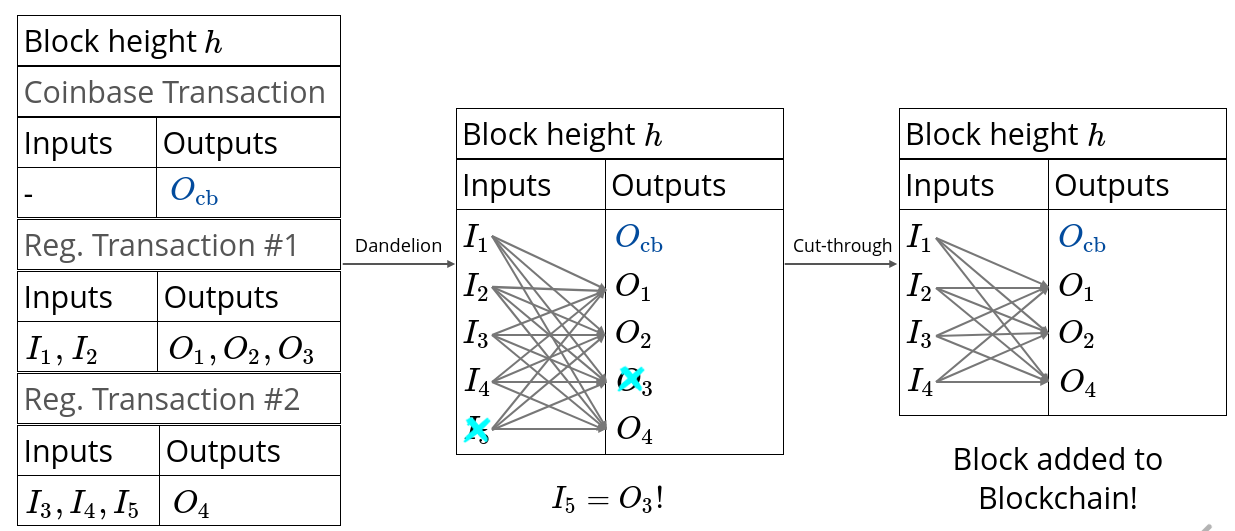
\includegraphics[width=0.92\textwidth]{Figures/block1.png}
  \centering
  \caption{A visual of the Dandelion protocol for transaction aggregation and the process of cut-through.
  Note that the coinbase outputs are denoted as $O_{\text{cb}}$ in blue colour.}
  \label{fig:dandelion}
\end{figure}

\begin{figure}[h!]
  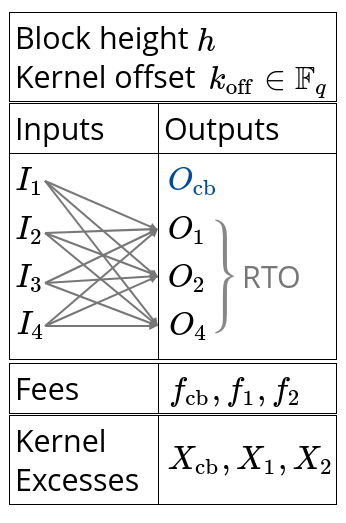
\includegraphics[width=0.27\textwidth]{Figures/block2.png}
  \centering
  \caption{Inclusion of kernels and fees in a Grin block. Note that the total number of transactions in a block are equal to the total number of kernels in a block.
  Also, $f_{\text{cb}} = 0$, the fees for coinbase transaction, for all Grin blocks.}
  \label{fig:kernels}
\end{figure}

% Each of these commitments refers to an output commitment in a previous block.An output is known as a \textit{coinbase} output if it is included by miners to store the mining reward and fees they earn
%during block mining. This transaction is known as \textit{coinbase} transaction.
%An output as a part of a regular transaction is known as \textit{transaction} output. 
%Each output is accompanied by a range proof to prove that it commits to an amount in the range $\{0,1,2, \dots,2^{64}-1\}$.  
%A Grin transaction consists of the following entities:
%\begin{enumerate}
%  \item[(i)] A vector of inputs serving as the sources of coins in the transaction. Each input is essentially an unspent output from some previous block.
%  \item[(ii)] A vector of outputs representing the destinations of coins in the transaction.
%  \item[(iii)] A vector of transaction kernels which are used in verification of transaction validity.
%\end{enumerate}
%A kernel is either a coinbase or a plain kernel according to the type of transaction.
%% A plain kernel is called as \textit{height-locked} kernel if the underlying transaction restricts its inclusion until a block at a specified height is mined.
%Each kernel contains the transaction fee and a \textit{kernel excess} which is a point on the curve of the form $xG$ where $x \in \mathbb{F}_n$.
%The kernel excess is accompanied by a Schnorr signature proving that it is of the form $xG$.
%% Transaction fee is included as a part of the kernel.
%
%A Grin block is characterized by a unique field called \textit{hash} which is SHA256 hash of its contents.
%% Each block contains the details of the Proof-of-Work used for mining.
%The inputs and outputs in a block are aggregated and we cannot distinguish between inputs and outputs of individual transactions.
%However, the total number of transactions in a block is equal to the number of kernels in that block.
%Suppose a block contains $L$ inputs $I_1, I_2, \dots, I_L$, $M$ outputs $O_1,O_2, \dots, O_M$
%and $N$ kernel excesses $X_1, X_2 \dots, X_N$ with individual fees $f_1, f_2 \dots, f_N$.
Refer to Figures \ref{fig:dandelion}, \ref{fig:kernels} for visual representation of a typical Grin block.
Let $\mathcal{I}_{\text{cb}} \subset \{1,2,\ldots,M\}$ be the set of indices corresponding to coinbase outputs and $\mathcal{I}_{\text{cb}}^c$ be the set of the remaining indices corresponding to RTOs. Let $\mathcal{I}_{\text{ck}} \subset \{1,2,\ldots,N\}$ be the set of indices corresponding to coinbase kernels and $\mathcal{I}_{\text{ck}}^c$ be the set of indices corresponding to regular transaction kernels. A valid block has to satisfy the following equations.
\begin{align}
  \sum_{i \in \mathcal{I}_{\text{cb}}} O_i - \left(\sum_{i=1}^{N}f_i\right)H - r H & = \sum_{i \in \mathcal{I}_{\text{ck}}} X_i,\\
  \sum_{i \in \mathcal{I}_{\text{cb}}^c} O_i + \left(\sum_{i=1}^{N}f_i\right)H - \sum_{i=1}^{L} I_i & = \sum_{i \in \mathcal{I}_{\text{ck}}^c} X_i + k_{\textnormal{off}}G.
  %\sum_{i=1}^{L} O_i + \left(\sum_{i=1}^{N}f_i\right)H - \sum_{i=1}^{M} I_i = \sum_{i=1}^{M} X_i + k_{\textnormal{off}}G
  \label{eqn:BlockValidity}
\end{align}
Here $r = 60\times 10^9$ is the block subsidy in nanogrin units.
As the right hand sides of both equations are commitments to the zero amount, the binding property of Pedersen commitments and the range proofs imply that
\begin{enumerate}
  \item[(i)] the total amount in the coinbase outputs of a block is $r + \sum_{i=1}^{N} f_i$ and
  \item [(ii)] the sum of the input amounts is equal to the sum of the transaction fees and RTO amounts.
\end{enumerate}
% The sum of coefficients of $H$ is zero in the above equation ensuring that no new coins are created.
%To see why (\ref{eqn:BlockValidity}) is enough to ensure validity of transactions, let
%$O_i = k_i^{\textnormal{out}}G + v_i^{\textnormal{out}}H$,
%$I_i = k_i^{\textnormal{in}}G + v_i^{\textnormal{in}}H$ and $X_i = x_iG$. Equation (\ref{eqn:BlockValidity}) holds only if the following hold
%\begin{align}
%  \sum_{i=1}^{M} v_i^{\textnormal{in}} &= \sum_{i=1}^{L} v_i^{\textnormal{out}} + \sum_{i=1}^{N}f_i \label{eqn:AmountEq} \\
%  \sum_{i=1}^{L} k_i^{\textnormal{out}} - \sum_{i=1}^{M} k_i^{\textnormal{in}} &= \sum_{i=1}^{N}x_i + k_{\textnormal{off}} \label{eqn:blindingFEq}
%\end{align}
%Equation (\ref{eqn:AmountEq}) implies that no new money was created and (\ref{eqn:blindingFEq}) implies that the coefficients of $G$ balance out.
%The reason for including $k_{\textnormal{off}}$ is to hide the relationship between the inputs and outputs in a block.
%If there were no kernel offset in a transaction, an adversary could attempt to deconstruct the individual transactions by trying combinations of inputs, outputs and kernels satisfying the transaction validity equation.
%
%A Grin block looks like a single transaction consisting of the aggregated inputs and outputs.
%If any output appears as an input in the same block, both of them are removed as they are not required for the block validation.
%Similarly, once an output is spent, it can be removed from the blockchain. 
%This process is known as \textit{cut-through} which improves scalability of Grin. 



% Revelio
\section{\textnormal{{\fontfamily{qag}\selectfont Revelio}} - A MimbleWimble Proof of Reserves Protocol}
\label{scn:revelio}

\R \cite{Dutta2019b} was the first proof of reserves protocol for MimbleWimble backed cryptocurrencies.
It uses non-interactive zero-knowledge (NIZK) proofs of knowledge for proving statements involving discrete logarithms which were originally introduced by \cite{Camenisch1997}.
% It presented a ring signature based approach to design proof of reserves proving statement of the form: an exchange owns $s$-out-of-$n$ outputs in a given anonymity set of size $n$.
% We briefly discuss Ring signature and Linkable Ring signature schemes used by \R and then present the idea of \Rw.

% \subsection{Ring Signatures}

% Ring Signatures were first introduced by Rivest et al. \cite{Rivest2001} in a paper titled `How to Leak a Secret'.
% Ring signatures make it possible to specify a set of possible signers without revealing which member actually produced the signature.
% They do not require any setup or coordination as against group signatures.



\subsection{Proving Statements About Discrete Logarithms}

Let $\G$ be a cyclic group of prime order $q$. Let $G, G^{\prime}, H$ be the generators of the group such that the discrete log relation between any two of them is assumed to be unknown.
We will use additive notation to be consistent with the notation used in \R paper.
\R uses three particular types of NIZK proofs of knowledge as defined below.
Let $\H \{0,1\}^{*} \rightarrow \Z_q $ be a cryptographic hash function modelled as a random oracle. 
The scalar pair $(\alpha, \beta) \in \Z_q^2$ is called as the representation of $X \in \G$ with respect to generators $G,H$ such that $X = \alpha G + \beta H$.
\begin{definition}
    A pair of scalars $(c,s) \in \Z_q^2$ is a NIZK proof of knowledge of the discrete log of an element $X \in \G$ with respect to a generator $G$ if they satisfy
    $$ c = \H(G,X,sG + cX). $$We will denote such a pair by $PoK\{\alpha \ | \ X = \alpha G \}$.
\end{definition}

\begin{definition}
    A triple of scalars $(c,s_1,s_2) \in \Z_q^3$ is a NIZK proof of knowledge and equality of the representations of $X,Y \in \G$ with respect to generator pairs $(G,H)$ and $(G^{\prime}, H)$ respectively if they satisfy
    $$ c = \H(S, s_1G+ s_2H+ cX,s_1G^{\prime} + s_2H + cX). $$where $S = (G\|G^{\prime}\|H\|X\|Y)$. We will denote such a triple by 
    \begin{equation*}
        PoK\{\underbrace{(\alpha, \beta)}_{\textsl{wit}} \ | \ \underbrace{X = \alpha G + \beta H \ \wedge \ Y = \alpha G^{\prime} + \beta H}_{\textsl{stmt}} \}.
    \end{equation*}
\end{definition}

\begin{definition}
    A 5-tuple of scalars $(c_1,c_2,s_1,s_2,s_3) \in \Z_q^5$ is a NIZK proof of either
    \begin{enumerate}
        \item[(i)] the knowledge and equality of the representations of $X,Y \in \G$ with respect to generator pairs $(G,H)$ and $(G^{\prime}, H)$ respectively OR
        \item[(ii)] knowledge of the discrete logarithm of the element $Y \in \G$ with respect to generator $G^{\prime}$, 
    \end{enumerate}  
    if they satisfy
    $$ c_1 + c_2 = \H(S, V_1, V_2, V_3). $$where $S = (G\|G^{\prime}\|H\|X\|Y)$ and 
    \begin{align*}
        V_1 &= s_1G+ s_2H+ c_1X, \\
        V_2 &= s_1G^{\prime}+ s_2H+ c_1X, \\
        V_3 &= s_3G^{\prime}+ c_2Y
    \end{align*}
    We will denote such a triple by 
    \begin{equation*}
        PoK\{\underbrace{(\alpha, \beta, \gamma)}_{\textsl{wit}} \ | \ \underbrace{(X = \alpha G + \beta H \ \wedge \ Y = \alpha G^{\prime} + \beta H) \vee (Y = \gamma G^{\prime})}_{\textsl{OR stmt}} \}.
    \end{equation*}
\end{definition}

\subsection{Main Idea of \textnormal{{\fontfamily{qag}\selectfont Revelio}}}

To generate a \R proof, an exchange chooses an anonymity set $\C_{\text{anon}} = (C_1, C_2, \dots, C_n)$ from the Grin blockchain.
Let the set of outputs owned by the exchange be $\C_{\text{own}} \subset \C_{\text{anon}}$. 
For $C_i \in C_{\text{own}}$, the exchange knows the blinding factor $k_i \in\Z_q$ such that $C_i = k_iG + a_iH$.
For each $C_i \in C_{\text{anon}}$, the exchange also publishes a tag $I_i$ defined as
\begin{equation}
    I_i = 
    \begin{cases}
        k_iG^{\prime} + v_iH & \text{if } C_i \in C_{\text{own}}\\
        y_iG^{\prime} & \text{if } C_i \notin C_{\text{own}}
    \end{cases}
\end{equation}
where $y_i = \H(k_{\text{exch}}, C_i)$ and $k_{\text{exch}}$ is a long-term secret key of the exchange.
The reason for such a definition of $y_i$ is that it needs to be a determinitic function of the chosen cover output $C_i$.
This is because we need to have consistent tag for a particular cover output $C_i$ appearing in $\C_{\text{anon}}$ over multiple \R proofs.
Additionally, the exchange publishes NIZK PoK $\sigma_i = (c_1^i,c_2^i, s_1^i, s_2^i, s_3^i)$ of the form 
\begin{equation*}
    PoK\{(\alpha, \beta, \gamma) \ | \ (C_i = \alpha G + \beta H \ \wedge \ I_i = \alpha G^{\prime} + \beta H) \vee (I_i = \gamma G^{\prime}) \}.
\end{equation*}
Lastly, the exchange claims that the commitment $C_{\text{assets}} = \sum_{i \in [n]} I_i$
is a Pedersen commitment to the total assets owned by the exchange.
Note that the tag list $(I_1, I_2, \dots, I_n)$ is used to check collusion among exchanges.
A \R proof verification involves checking of any matches in tags of different exchanges and verification of the NIZK PoKs $\sigma_i \ \forall i \in [n]$.

\subsection{Drawbacks of \textnormal{{\fontfamily{qag}\selectfont Revelio}}}

The size of a \R proof is $5n$ elements in $\Z_q$ and $n+1$ elements in $\G$.
Privacy provided by \R for exchange-owned outputs directly depends on the number of cover addresses used.
An exchange would ideally like to have the entire UTXO set as the anonymity set. 
Since the proof sizes in \R increase linearly
with the size of $C_{\text{anon}}$, setting $C_{\text{anon}}$ to be equal
to the whole UTXO set is not a scalable strategy.

The collusion-resistance property of \R works only
if all the exchanges generate their proofs using the same
blockchain state.
Cryptographically enforcing simultaneous proof generation is necessary to avoid cheating by exchanges.
Both of the above drawbacks led us to the development of \RB which solves the above drawbacks with a higher computational cost.
We describe \RB in the next chapter. 


%%% Local Variables: 
%%% mode: latex
%%% TeX-master: "../mainrep"
%%% End: 


\chapter{Materials and Methods}

\section{Including Figures}




%%% Local Variables: 
%%% mode: latex
%%% TeX-master: "../mainrep"
%%% End: 

\chapter{Results and Discussions}


\section{Including Tables}

Tables are to be used in a special environment so that they have a
Number, caption and appear in the list of tables.
Table~\ref{tab:samtab} is a sample table. In the case of tables, it is
a convention to write the caption above the table.  Note that in the
case of figures the caption appears below the figure.

\begin{table}[tbp]
  \centering
    \caption{Physical properties of the materials used.}
    \label{tab:samtab}
    \begin{tabular}{ll}
      \toprule 
      Property & Value \\
      \midrule
      Particle Density, $\rho_{\mathrm{p}}$ & 2500 kg/m$^{3}$ \\
      Viscosity, $\eta_{\mathrm{s}}$& 1 $\times 10^{-3}$ Pa-s \\
      \bottomrule \\
    \end{tabular}  
\end{table}

%%% Local Variables: 
%%% mode: latex
%%% TeX-master: "../mainrep"
%%% End: 


%****************************************************************
%                         Appendices                           
%****************************************************************
%% Additional, supporting material, such as codes, derivations, etc., can be placed in the appendix
\appendix
\chapter{Supporting Material}

%******************************************************************
%                         Bibliography or References          
%******************************************************************  
\bibliography{mylit}

%*******************************************************************
%                         List of publications               
%******************************************************************
%%%
% \makeheadtoc{List of Publications}
% \bibliographystylePub{ieeetr}
% \bibliographyPub{pub}
% \nocitePub{*}
\listofpublications

% Hard coding as of now
\begin{enumerate}[label={[\arabic*]}, leftmargin=\parindent, align=left, labelwidth=\parindent,labelsep=0pt]
    \item S. Bagad and S. Vijayakumaran, ``On the Confidentiality of Amounts in Grin,'' in \textit{Crypto Valley Conference on Blockchain Technology} \textit{(CVCBT)}, 2020.
    \item S. Bagad and S. Vijayakumaran, ``Performance Trade-offs in Design of MimbleWimble Proofs of Reserves,'' in \textit{IEEE European Symposium on Security and Privacy Workshops (EuroS\&PW)}, 2020.
\end{enumerate}


% \bibliographystylePub{ieeetr}
% \bibliographyPub{pub}
% \nocitePub{*}








%%======================================================================
%%% Local Variables: 
%%% mode: latex
%%% TeX-master: "../mainrep"
%%% End: 







            

%*******************************************************************
%                        Acknowledgements                    
%******************************************************************* 
%%%
\acknowledgments

I would like to express my deepest appreciation and gratitude to my guide Prof.
Saravanan Vijayakumaran for his guidance and constant supervision and help throughout the last 18 months. 
His insightful suggestions and comments have time and again helped me get a more in-depth understanding of the field.
His most valuable lesson for me, from amongst many others, was to be persistent especially in times when things are not going as planned. 
Not only did he offer consistent assistance with regards to the academic work but also gave invaluable suggestions in helping me carve out my career path. 
I also thank the Bharti Centre for Communication at IIT Bombay and Vibha ma'am particularly for providiting necessary logistical support.
Thanks are also due to Arijit Dutta of IIT, Bombay for his many useful remarks and discussions about the project and otherwise. 
I also acknowledge the help offered by my brother Piyush Bagad (Wadhwani AI) in understanding Python as well as in running simulations. 
I would also like to thank my dear friend Madhura Pawar for her constant encouragement
which helped me work towards my goal even when things weren't working out.
Finally, I express gratitude towards my family for giving me the opportunities and freedom in choosing research as my career.





\signature{\today}
%\signature[Indian Institute of Technology Bombay]{\today}

%========================================================================

%%% Local Variables: 
%%% mode: latex
%%% TeX-master: "../mainrep"
%%% End:            


% GAME OVER
%*******************************************************************
\end{document}

%%% Local Variables: 
%%% mode: latex
%%% TeX-master: t
%%% End: 
